% Created with jtex v.1.0.4
\documentclass{article}
\usepackage{arxiv}

\usepackage[utf8]{inputenc} % allow utf-8 input
\usepackage[T1]{fontenc}    % use 8-bit T1 fonts
\usepackage{hyperref}       % hyperlinks
\usepackage{url}            % simple URL typesetting
\usepackage{datetime}       % show dates in the title block
\usepackage{booktabs}       % professional-quality tables
\usepackage{amsfonts}       % blackboard math symbols
\usepackage{nicefrac}       % compact symbols for 1/2, etc.
\usepackage{microtype}      % microtypography
\usepackage{graphicx}
\usepackage{natbib}
\usepackage{doi}
\usepackage{xcolor}

%%%%%%%%%%%%%%%%%%%%%%%%%%%%%%%%%%%%%%%%%%%%%%%%%%
%%%%%%%%%%%%%%%%%%%%  imports  %%%%%%%%%%%%%%%%%%%
\usepackage{amsmath}
%%%%%%%%%%%%%%%%%%%%%%%%%%%%%%%%%%%%%%%%%%%%%%%%%%

\hypersetup{colorlinks = true,
linkcolor = purple,
urlcolor  = blue,
citecolor = cyan,
anchorcolor = black}

\title{Attractor states of the functional brain connectome orchestrate large-scale brain dynamics}

\newdate{articleDate}{28}{8}{2023}
\date{\displaydate{articleDate}}

\makeatletter
\let\@fnsymbol\@arabic
\makeatother

\author{Robert Englert\\
Department of Diagnostic and Interventional Radiology and Neuroradiology,  University Medicine Essen, Germany\\\AND
Balint Kincses\\
Department of Neurology, University Medicine Essen, Germany\\\AND
Raviteja Kotikalapudi\\
Department of Neurology, University Medicine Essen, Germany\\\AND
Giuseppe Gallitto\\
Department of Neurology, University Medicine Essen, Germany\\\AND
Jialin Li\\
Department of Neurology, University Medicine Essen, Germany\\Max Planck School of Cognition, Leipzig, Germany\\\AND
Kevin Hoffschlag\\
Department of Neurology, University Medicine Essen, Germany\\\AND
Choong-Wan Woo\\
Center for Neuroscience Imaging Research, Institute for Basic Science, Suwon, South Korea\\Department of Biomedical Engineering, Sungkyunkwan University, Suwon, South Korea\\\AND
Tor D. Wager\\
Department of Psychological and Brain Sciences, Dartmouth College, Hanover, NH, USA\\\AND
Dagmar Timmann\\
Department of Neurology, University Medicine Essen, Germany\\Center for Translational Neuro- and Behavioral Sciences (C-TNBS), University Medicine Essen, Germany\\\AND
Ulrike Bingel\\
Department of Neurology, University Medicine Essen, Germany\\Center for Translational Neuro- and Behavioral Sciences (C-TNBS), University Medicine Essen, Germany\\\AND
\href{https://orcid.org/0000-0002-2942-0821}{
\includegraphics[scale=0.06]{orcid.pdf}}\hspace{1mm}Tamas Spisak\footnotemark[1]\\
Department of Diagnostic and Interventional Radiology and Neuroradiology,  University Medicine Essen, Germany\\Center for Translational Neuro- and Behavioral Sciences (C-TNBS), University Medicine Essen, Germany\\\AND
for the Alzheimer’s Disease Neuroimaging Initiative\\
One of the dataset used in preparation of this article were obtained from the Alzheimer’s Disease Neuroimaging Initiative (ADNI)  database (adni.loni.usc.edu). As such, the investigators within the ADNI contributed to the design and implementation of ADNI and/or provided data but did not participate in analysis or writing of this report. A complete listing of ADNI investigators can be found at: http://adni.loni.usc.edu/wp-content/uploads/how_to_apply/ADNI_Acknowledgement_List.pdf\\}

% Uncomment to override  the `A preprint' in the header
\renewcommand{\headeright}{Preprint}
\renewcommand{\undertitle}{}
\renewcommand{\shorttitle}{ConnAttractor Preprint}

%% Add PDF metadata to help others organize their library
%% Once the PDF is generated, you can check the metadata with
%% $ pdfinfo template.pdf
\hypersetup{
pdftitle={\@title},
pdfsubject={},
pdfauthor={\@author},
pdfkeywords={},
addtopdfcreator={Written in Curvenote}
}

\begin{document}
\maketitle
\footnotetext[1]{Correspondence to: tamas.spisak@uk-essen.de}

\begin{abstract}
Understanding large-scale brain dynamics is a grand challenge in neuroscience.
We propose functional connectome-based Hopfield artificial neural networks (FCHNs) as a model of recurrent, dynamic, macro-scale activity flow among brain regions.
FCHNs are neither optimized to mimic certain brain characteristics nor trained to solve specific tasks, but simply initialized with the empirical functional connectome.
The FCHN framework identifies neurobiologically meaningful attractor states and provides a model for how these constrain brain dynamics.
Analyses of 8 distinct datasets (N$\approx$2000) demonstrate that FCHNs can accurately reconstruct and predict brain dynamics under a wide range of conditions, including resting state and task-induced activity changes, as well as various brain disorders.
FCHNs establish a conceptual link between connectivity and activity and offer a simple, robust, and highly interpretable computational alternative to the conventional descriptive approaches for investigating brain function.
FCHNs have the potential to unveil the mechanisms underlying altered large-scale brain dynamics in a wide range of clinical conditions and hold promise for identifying potential targets for novel treatment approaches.
\end{abstract}

\keywords{}

\textbf{Key Points:}

\begin{itemize}
\item We present a simple yet powerful computational model for large-scale brain dynamics
\item The model uses a functional connectome-based Hopfield artificial neural network (FCHN) architecture to compute recurrent "activity flow" trough the functional brain connectome
\item FCHNs accurately reconstruct the dynamic repertoire of the brain in resting conditions
\item FCHNs conceptualize both task-induced and pathological changes in brain activity as a shift in these dynamics
\item Our approach is validated through eight studies involving approximately 2000 participants
\end{itemize}

\subsection{Introduction}\label{Introduction}

Brain function is characterized by the continuous activation and deactivation of anatomically distributed neuronal
populations.
While the focus of related research is often on the direct mapping between activity changes in a single brain
area and a specific task or condition, in reality, regional activation never seems to occur in isolation
\citep{bassett2017network}.

Irrespective of the presence or absence of explicit stimuli, brain regions appear to work in concert, giving rise to a
rich and spatiotemporally complex fluctuation \citep{gutierrez2019infraslow}.
This fluctuation is neither random, nor stationary over time \citep{liu2013time, zalesky2014time}.
It exhibits quasi-periodic properties \citep{thompson2014quasi}, with a limited number of
recurring patterns known as "brain states" \citep{greene2023everyone, vidaurre2017brain, liu2013time, richiardi2011decoding}.

From hidden Markov models, to point-process analyses, a wide variety of descriptive techniques have been previously
employed to characterize whole-brain dynamics \citep{smith2012temporally, vidaurre2017brain, liu2013time, chen2018human}.
These efforts have provided accumulating evidence not only for the existence of dynamic brain states but also for their clinical
significance \citep{hutchison2013dynamic, barttfeld2015signature, meer2020movie}.
However, the underlying driving forces remain elusive due to the descriptive nature of such studies.

Questions regarding the mechanisms, that cause these remarkable dynamics, can be addressed through computational models, which have the potential to shift our understanding from mere associations to causal explanations.
Conventional computational approaches attempt to solve this puzzle by going all the way down to the biophysical properties of single neurons, and aim to construct a model of larger neural populations, or even the entire brain
\citep{breakspear2017dynamic}.
These approaches have shown numerous successful applications \citep{murray2018biophysical, kriegeskorte2018cognitive, heinz2019towards}.
However, the estimation of the vast number of free parameters in such models presents a grand challenge, hampering the ability of these techniques to effectively bridge the gap between explanations at the level of single neurons and the complexity of behavior \citep{breakspear2017dynamic}. As a result, several recent approaches have opted to trade biophysical detail for computational simplicity. They utilize phenomenological, coarse-grained models \citep{schiff1994controlling, papadopoulos2017development} of neural activity, like linear network control theory  \citep{luppi2023transitions, chiem2021structure, gu2017optimal, scheid2021time}, to gain insights into how structural connectivity constrains brain dynamics.

Another approach, the so-called "neuroconnectionism" \citep{doerig2023neuroconnectionist} shifts the emphasis from "biophysical fidelity" of models to "cognitive/behavioral fidelity"
\citep{kriegeskorte2018cognitive}, by using artificial neural networks (ANNs) that are trained to
perform various tasks, as brain models. While this novel paradigm has already made significant contributions to expanding our understanding of the general computational principles of the brain (see \citep{doerig2023neuroconnectionist}, the need to train ANNs for specific tasks inherently limits their ability to explain the spontaneous, and largely task-independent, macro-scale dynamics of neural activity \citep{richards2019deep}.

Here we propose a novel approach that combines phenomenological computational modeling and neuroconnectionism to investigate brain dynamics.
We utilize an artificial neural network (ANN) as a high-level computational model of the brain.
However, we do not explicitly train our ANN for a specific task. Instead, we employ a neurobiologically well motivated ANN architecture, which shares main principles with phenological models, with its weights set empirically, with data based on the "activity flow" \citep{cole2016activity, ito2017cognitive}
across regions within the functional brain connectome, as measured with functional magnetic resonance imaging
(fMRI, Figure~\ref{concept}B).

Specifically, we employ a continuous-space Hopfield neural network (HNN) \citep{hopfield1982neural, krotov2023new} that, based on the topology of the functional connectome, establishes an "energy" level for any arbitrary activation patterns and determines a "trajectory of least action" towards one of the finite number of stable patterns, known as \textit{attractor states}, that minimize this energy.
If the stochastic nature of neural activity is approximated by adding weak noise to the system, it does not reach equilibrium anymore (i.e. it does not converge to an attractor state).
Instead, it traverses extensive regions of the state space, with dynamics influenced by multiple attractor states, arising form the topology of the functional brain connectome (Figure~\ref{concept}C). Through this walk across the state space, our model offers a natural explanation for brain state dynamics.

\begin{figure}[!htbp]
\centering
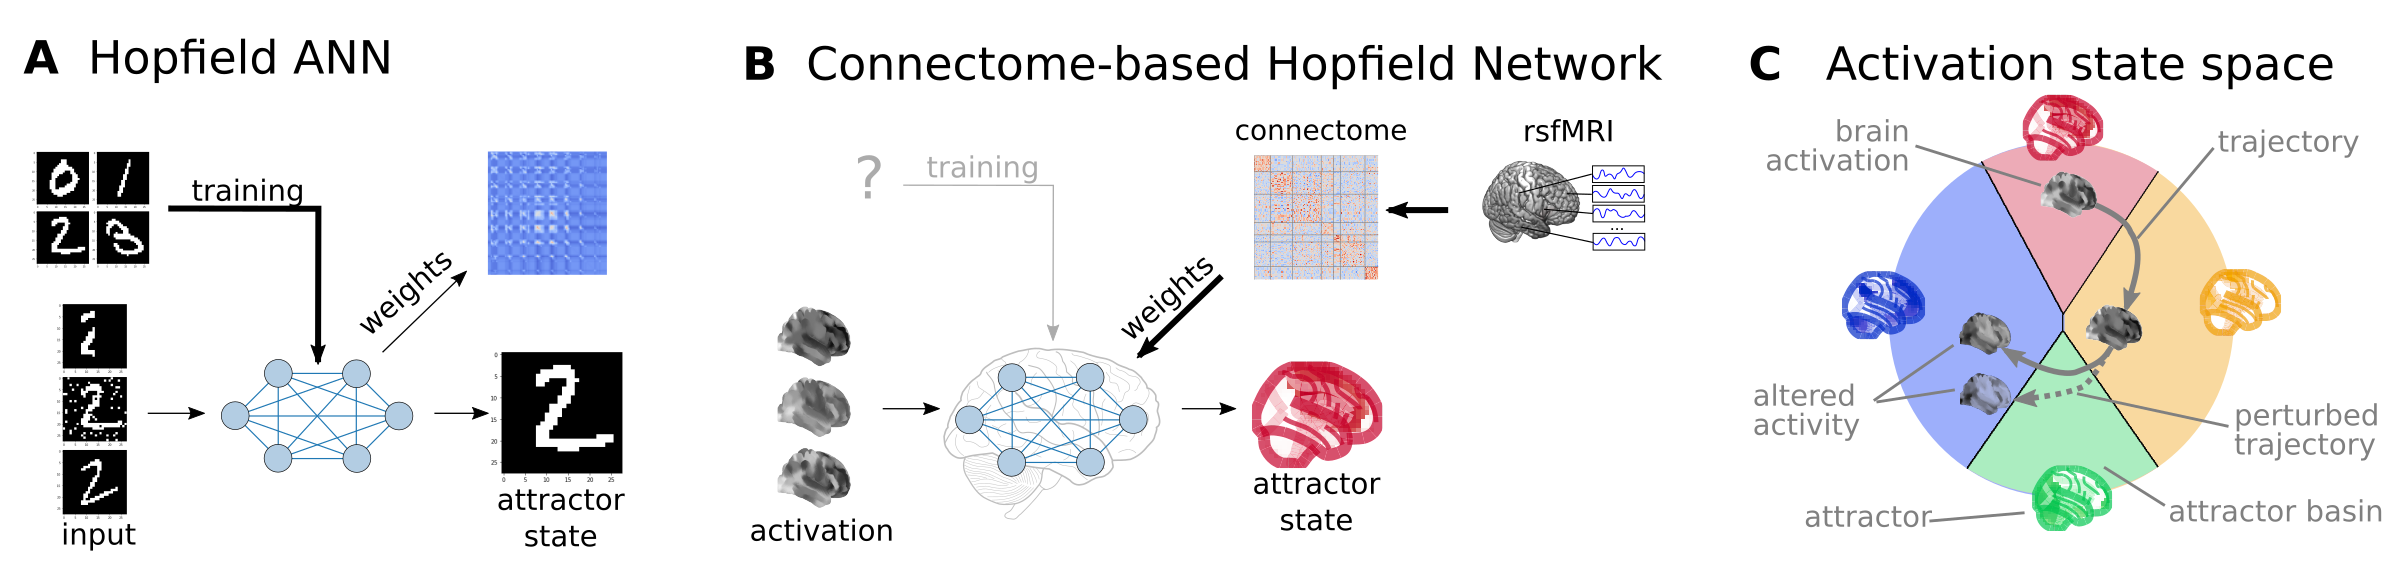
\includegraphics[width=0.7\linewidth]{files/concept-bf588273323d07e9d5e6c1a50ee97ed4.png}
\caption[]{\textbf{Connectome-based Hopfield networks as models of macro-scale brain dynamics.} \newline
\newline

\textbf{A} Hopfield artificial neural networks (HNNs)  are a form of recurrent artificial neural networks that serve as content-addressable
("associative") memory systems. Hopfield networks can be trained to store a finite number of patterns (e.g. via
Hebbian learning a.k.a. "fire together -  wire together"). During the training procedure, the weights of the HNN are trained so that the stored
patterns become stable attractor states of the network. Thus, when the trained network is presented partial, noisy or corrupted
variations of the stored patterns, it can effectively reconstruct the original pattern via an iterative relaxation
procedure that converges to the attractor states.
\textbf{B} We consider regions of the brain as nodes of a Hopfield network. Instead of training the Hopfield network to
specific tasks, we set its weights empirically, with the interregional activity flow estimated via functional
brain connectivity. Capitalizing on strong analogies between the relaxation rule of Hopfield networks and the
activity flow principle that links activity to connectivity in brain networks, we propose the resulting
functional connectome-based Hopfield neural network (FCHN) as a computational model for macro-scale brain dynamics.\newline
\textbf{C} The proposed computational framework assigns an energy level, an attractor state and a position in a
low-dimensional embedding to brain activation patterns. Additionally, it models how the entire state-space of viable
activation patterns is restricted by the dynamics of the system and how alterations in activity and/or connectivity
modify these dynamics.}
\label{concept}
\end{figure}

In this simplistic yet powerful framework, both spontaneous and task-induced brain dynamics can be conceptualized as an intricate, high-dimensional path that meanders on the energy landscape, restricted by the "gravitational pull" of the attractors states.
The framework provides a generative model for both resting state and task-related brain dynamics, offering novel
perspectives on the mechanistic origins of resting state brain states and task-based activation maps.

In the present work, we first explore the attractor states of the functional brain connectome and construct a
low-dimensional representation of the energy landscape.
Subsequently, we rigorously test the proposed model through a series of experiments, conducted on data obtained
from 8 experimental and clinical studies, encompassing a total of n$\approx$2000 individuals.
These analyses evaluate the robustness and replicability of the proposed approach and test its ability to reconstruct
various characteristics of resting state brain dynamics, as well as its capacity to detect and explain changes induced
by experimental tasks or alterations characteristic to brain disorders.

These experiments provide converging evidence for the validity of connectome-based Hopfield neural networks as models
of brain dynamics, and highlight their potential to provide a fresh perspective on a wide range of research questions
in basic and translational neuroscience.

\subsection{Main}\label{Main}

\subsubsection{Connectome-based Hopfield network as a model of brain dynamics}\label{Connectome-based Hopfield network as a model of brain dynamics}

First, we explored the attractor states of the functional connectome in a sample of n=41 healthy young
participants (Table~\ref{tab-samples}). We estimated interregional activity flow \citep{cole2016activity, ito2017cognitive}
as the study-level average of regularized partial correlations among the resting state fMRI timeseries of m = 122
functionally defined brain regions (BASC brain atlas, see Methods for details). We then used the standardized
functional connectome as the $w_{ij}$  weights of a continuous-state Hopfield network
\citep{hopfield1982neural, koiran1994dynamics} consisting of $m$ neural units, each having an activity
$a_i \in [ -1,1] \subset \mathbb{R})$. Hopfield networks can be initialized by an arbitrary activation pattern (consisting of
$m$ activation values) and iteratively updated (i.e. "relaxed") until convergence to one of the finite attractor states is reached. The relaxation procedure is based in a simple rule; in each iteration, the activity of a region is constructed as the weighted average of the activities of all other regions, with weights defined by the connectivity between them.
This can be expressed by the following equation:

\begin{equation}
\label{hopfield-update}
\dot{a}_i = S(\beta \sum_{j=1}^m w_{ij}a_j - b_i)
\end{equation}

where $\dot{a}_i$ is the activity of neural unit $i$ in the next iteration and $S(a_j)$ is the sigmoidal activation
function ($S(a) = tanh(a)$ in our implementation) and $b_i$ is the bias of unit $i$ and $\beta$ is the so-called temperature parameter. For the sake of simplicity, we set $b_i=0$ in all our experiments. We refer to this architecture as a functional connectivity-based Hopfield neural network (FCHN). Importantly, the relaxation of a FCHN model can be conceptualized as the repeated
application of the activity flow principle \citep{cole2016activity, ito2017cognitive} , simultaneously for all
regions: $\dot{a}_i = \sum_{j=1}^m w_{ij}a_j$. The update rule also exhibits strong analogies with the inner workings
of neural mass models \citep{breakspear2017dynamic} as applied e.g. in dynamic causal modeling(see Discussion for
further details).

Hopfield networks assign an energy value to each possible activity configuration (see Methods), which decreases during
the relaxation procedure until reaching an equilibrium state with minimal energy (Figure~\ref{attractors}A, top panel,
\citep{hopfield1982neural, koiran1994dynamics}.
We used a large number of random initializations to obtain all possible attractor states of the connectome-based
Hopfield network in study 1 (Figure~\ref{attractors}A, bottom panel).

\begin{figure}[!htbp]
\centering
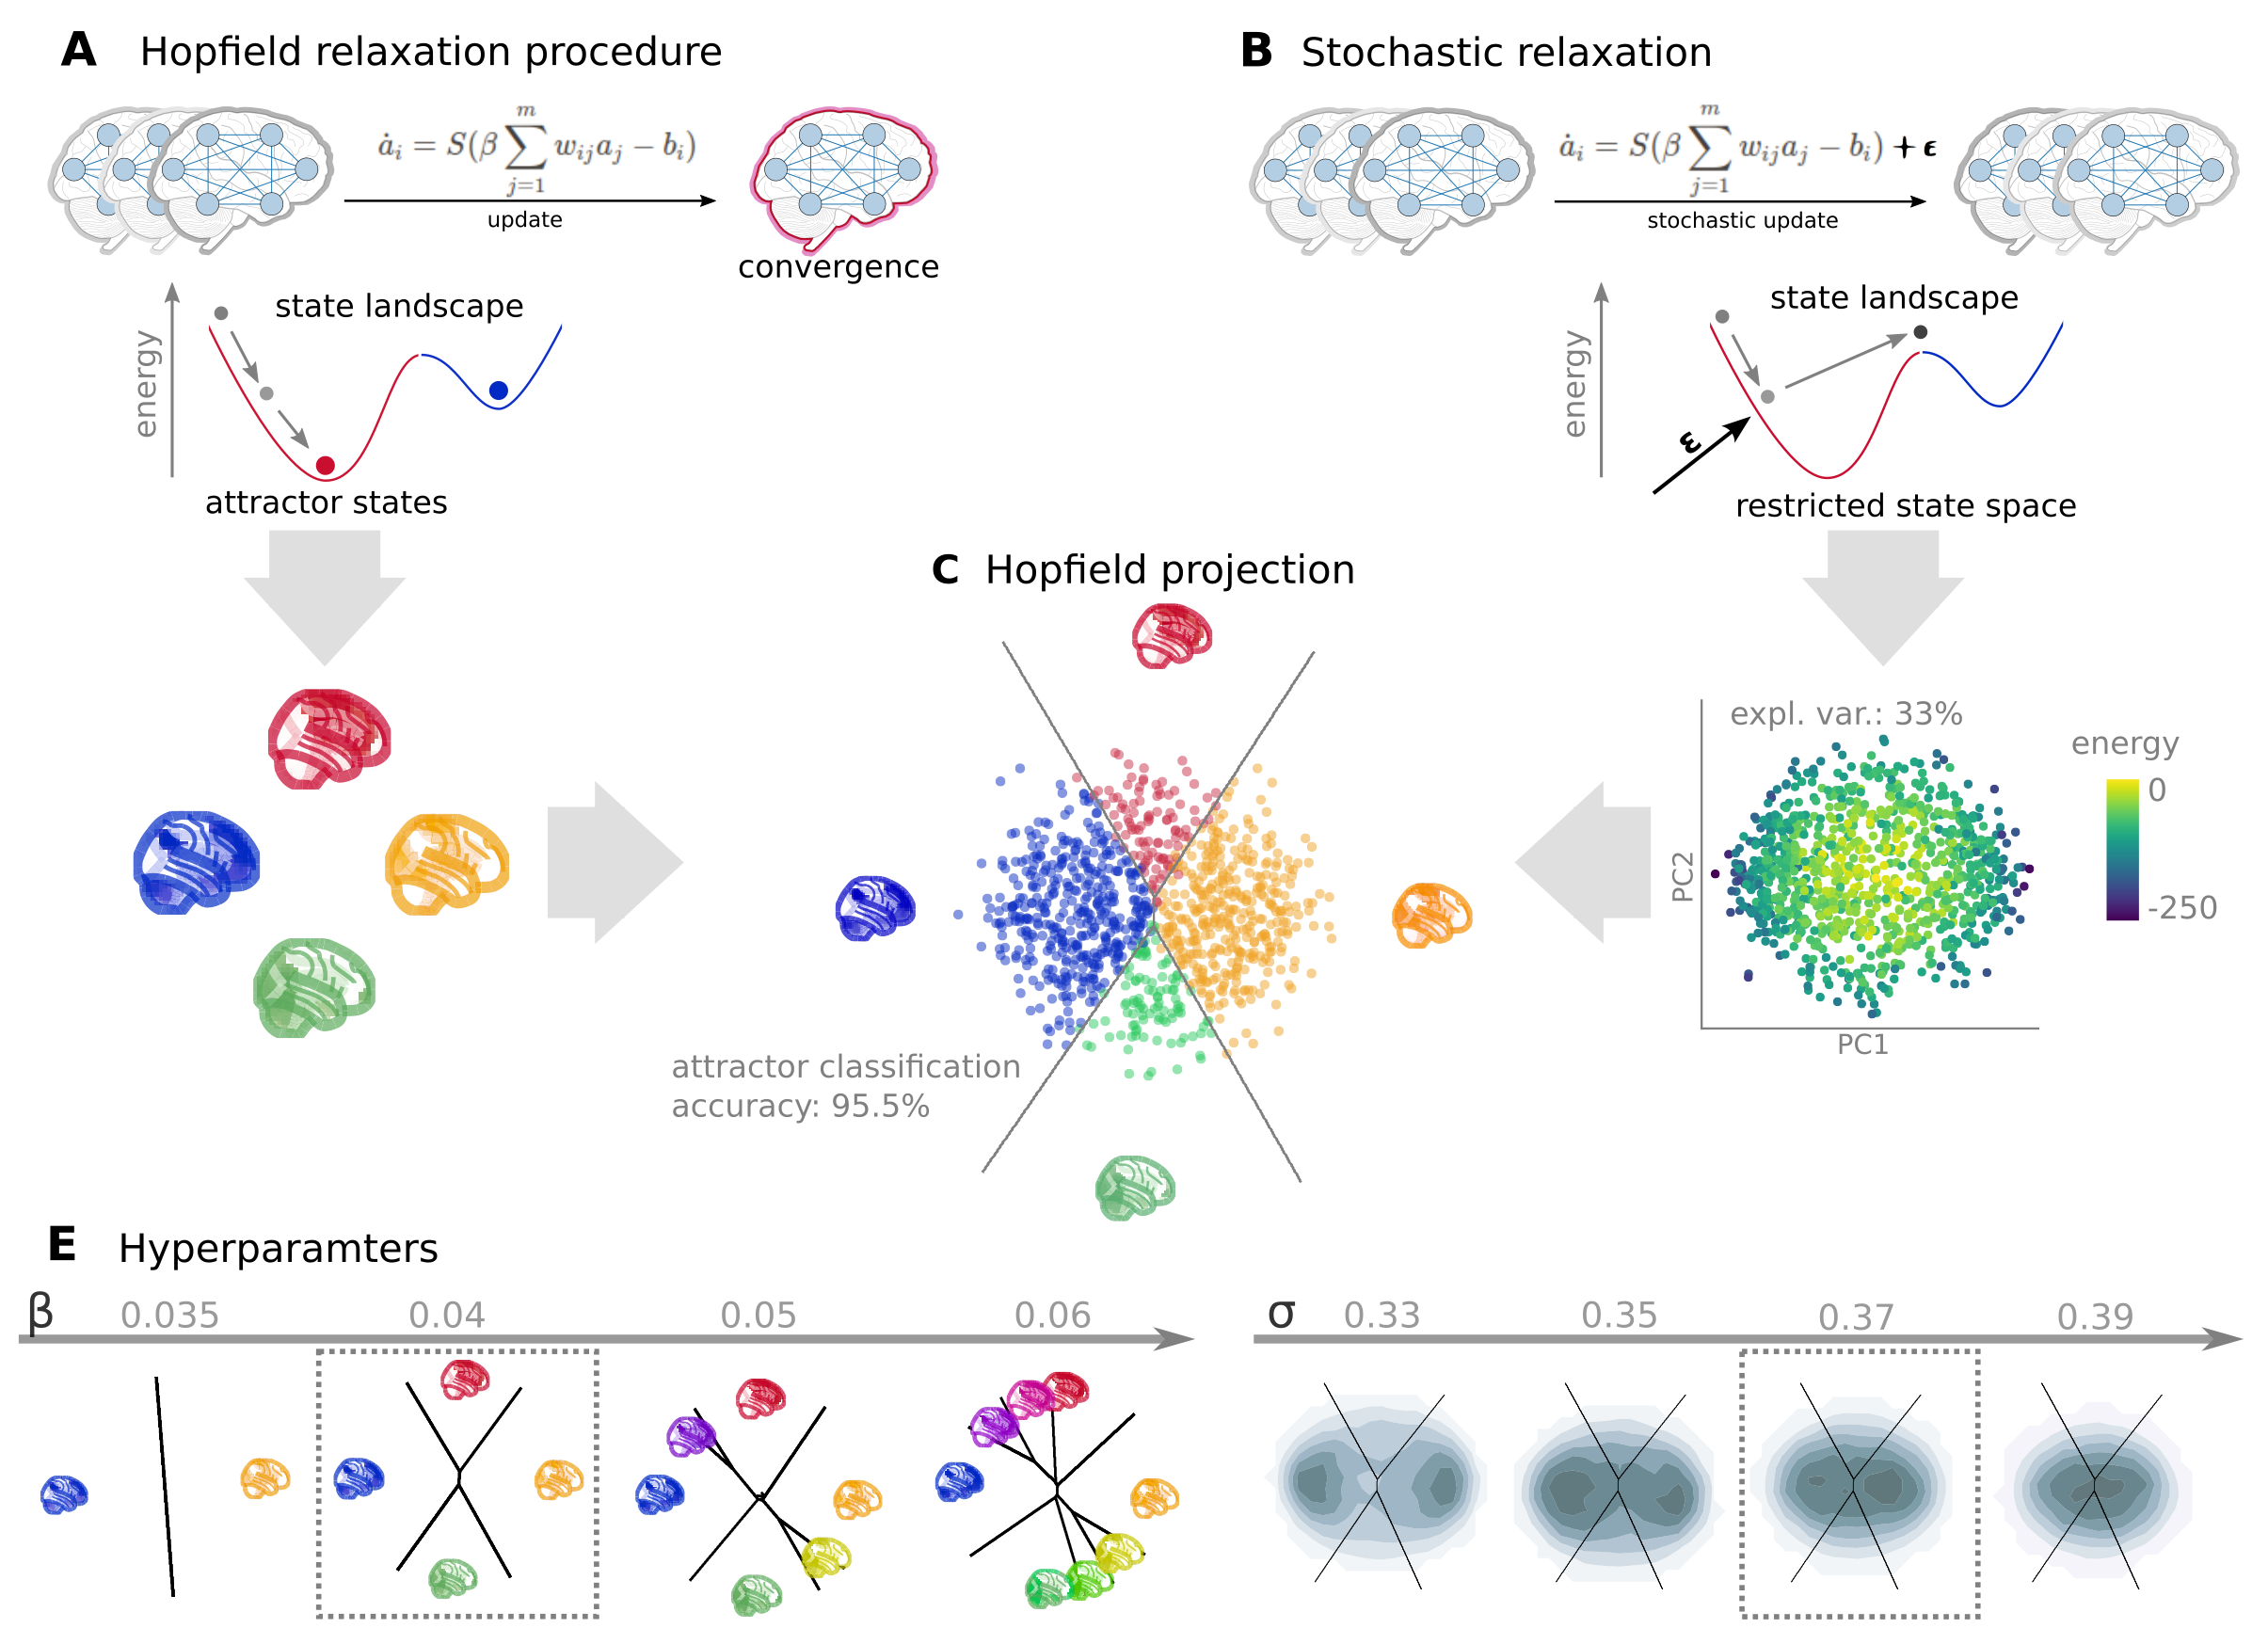
\includegraphics[width=0.7\linewidth]{files/embedding_method-2a5fac4fd92ac4c692050050214094e5.png}
\caption[]{\textbf{Attractor states and state-space dynamics of connectome-based Hopfield networks} \newline
\newline

\textbf{A} Top: During so-called relaxation procedure, activities in the nodes of an FCNN model are iteratively updated based on the activity of all other regions and the connectivity between them. The energy of a
connectome-based Hopfield network decreases during the relaxation procedure until reaching an equilibrium state with
minimal energy, i.e. an attractor state. Bottom: Four attractor states of the CHNN derived from the
group-level functional connectivity matrix from Table~\ref{tab-samples} (n=44).
\textbf{B} Top: Similarly to stochastic dynamic causal modeling, in presence of weak noise (stochastic update), the system
does not converge to equilibrium anymore. Instead, the system transverses on the state landscape in a way
restricted by the topology of the connectome and the "gravitational pull" of the attractor states. Bottom: We sample
the state space by running the stochastic relaxation procedure for an extended amount of time (e.g. 100.000 consecutive
stochastic updates), each point representing a possible activation configuration (state). To construct a
low-dimensional representation of the state space, we take the first two principal components of the simulated activity
patterns. The first two principal components explain approximately 55-85\% of the variance of state energy (depending
on the noise parameter $\sigma$, see Supplementary Material \textbf{X}).
\textbf{C} We map all states of the state space sample to their corresponding attractor state, with the conventional
Hopfield relaxation procedure (A). The four attractor states are also visualized in their corresponding position on the
PCA-based projection. The first two principal components yield a clear separation of the attractive state basins
(cross-validated classification accuracy: 95.5\%, Supplementary Material \textbf{X}). We refer to the resulting visualization
as the Hopfield projection and use it to visualize FCHN-derived and empirical brain dynamics throughout the rest of
the manuscript.
\textbf{E} At its simplest form, the FCHN framework entails only two free hyperparameters: the temperature parameter
$\beta$ (left) that controls the number of attractor states and the noise parameter of the stochastic relaxation
$\sigma$. To avoid overfitting these parameters to the empirical data, we set $\beta=0.04$ and $\sigma=0.37$ for the
rest of the paper  (dotted boxes).}
\label{attractors}
\end{figure}

Consistent with theoretical expectations, we observed that increasing the temperature parameter $\beta$ led to an
increasing number of attractor states (Figure~\ref{attractors}E, left), appearing in symmetric pairs
(i.e. $a_i^{(1)} = -a_i^{(2)}$). For simplicity, we set the temperature parameter for the rest of the paper to a value
resulting in 4 distinct attractor states ($\beta=0.4$).

Connectome-based Hopfield networks, without any modifications, always converge to an equilibrium state.
To incorporate stochastic fluctuations in neuronal activity \citep{robinson2005multiscale}, we introduce weak
Gaussian noise to the FCHN relaxation procedure. This procedure, referred to as stochastic relaxation, prevents the
system from reaching equilibrium and, somewhat similarly to stochastic DCM \citep{daunizeau2012stochastic}, induces
complex system dynamics  (equivalent to brain activity fluctuations in our framework). Such a system may traverse extensive
regions of the state space, in a way largely shaped by the "gravitational pull" (the so-called "basins") of multiple attractor states (Figure~\ref{attractors}B).

We hypothesise that the resulting dynamics capture essential characteristics of spontaneous activity fluctuations in
the brain and can serve as a valuable generative computational model for large-scale brain dynamics. To sample the
resulting state space, we obtained 100,000 iterations of the stochastic relaxation procedure with a Hopfield network
initialized with the mean functional connectome in study 1. Next, in order to enhance interpretability, we conducted a
principal component analysis (PCA) on the resulting state space sample and obtained the first two principal components.
These components were used to construct a low-dimensional embedding (Figure~\ref{attractors}B, bottom plot).

The PCA embedding exhibited high consistency across different values of $\beta$ and $\sigma$ (Figure~\ref{attractors}E).
For all subsequent analyses, we set $\sigma=0.37$, which was determined through a coarse optimization procedure aimed
at reconstructing the bimodal distribution of empirical data in the same projection (Figure~\ref{attractors}E,
see Methods for details). On the low-dimensional embedding, which we refer to as the \textit{FCHN projection}, we observed
a clear separation of the attractor states (Figure~\ref{attractors}C), with the two symmetric pairs of attractor states
located at the extremes of the first and second PC.
To map the attractor basins on the space spanned by the first two PCs (Figure~\ref{attractors}C), we obtained the attractor state of each point visited during the stochastic relaxation and fit a multinomial logistic regression model to predict the attractor state from the first two PCs.
The resulting model accurately predicted attractor states of arbitrary brain activity patterns, achieving a cross-validated accuracy of 96.5\%.
The attractor basins were visualized by using the decision boundaries obtained from this model. (Figure~\ref{attractors}C). We propose the 2-dimensional FCHN projection depicted on (Figure~\ref{attractors}C) as a simplified representation of brain dynamics, and use it as a basis for all subsequent analyses in this work.

\subsubsection{Reconstruction of resting state brain dynamics}\label{Reconstruction of resting state brain dynamics}

The spatial patterns of the obtained attractor states exhibit high neuroscientific relevance and closely resemble previously described large-scale brain systems. (Figure~\ref{rest-validity}A). The first pair of attractors (mapped on PC1, horizontal axis) resemble the two complementary ``macro'' systems described, among others, by \citet{golland2008data} and \citet{cioli2014differences} as well as the two "primary" brain states observed by \citet{chen2018human} and the dysphoric and anxiosomatic clusters that have recently been proposed as targets for circuit-based neuromodulation by \citet{siddiqi2020distinct}. A common interpretation of these two patterns is that they represent (i) an ``extrinsic'' system
which exhibits a stronger direct connection to the immediate sensory environment and (ii) an "intrinsic" system, whose
activity is primarily associated with dynamic changes in higher-level internal context and closely linked to the default
mode network.
The other pair of attractors spans an orthogonal axis connecting regions that are commonly associated
with perception--action cycles \citep{fuster2004upper} and recruits regions associated with active inference (e.g. motor cortices) and perceptual inference (e.g visual cortices).

\begin{figure}[!htbp]
\centering
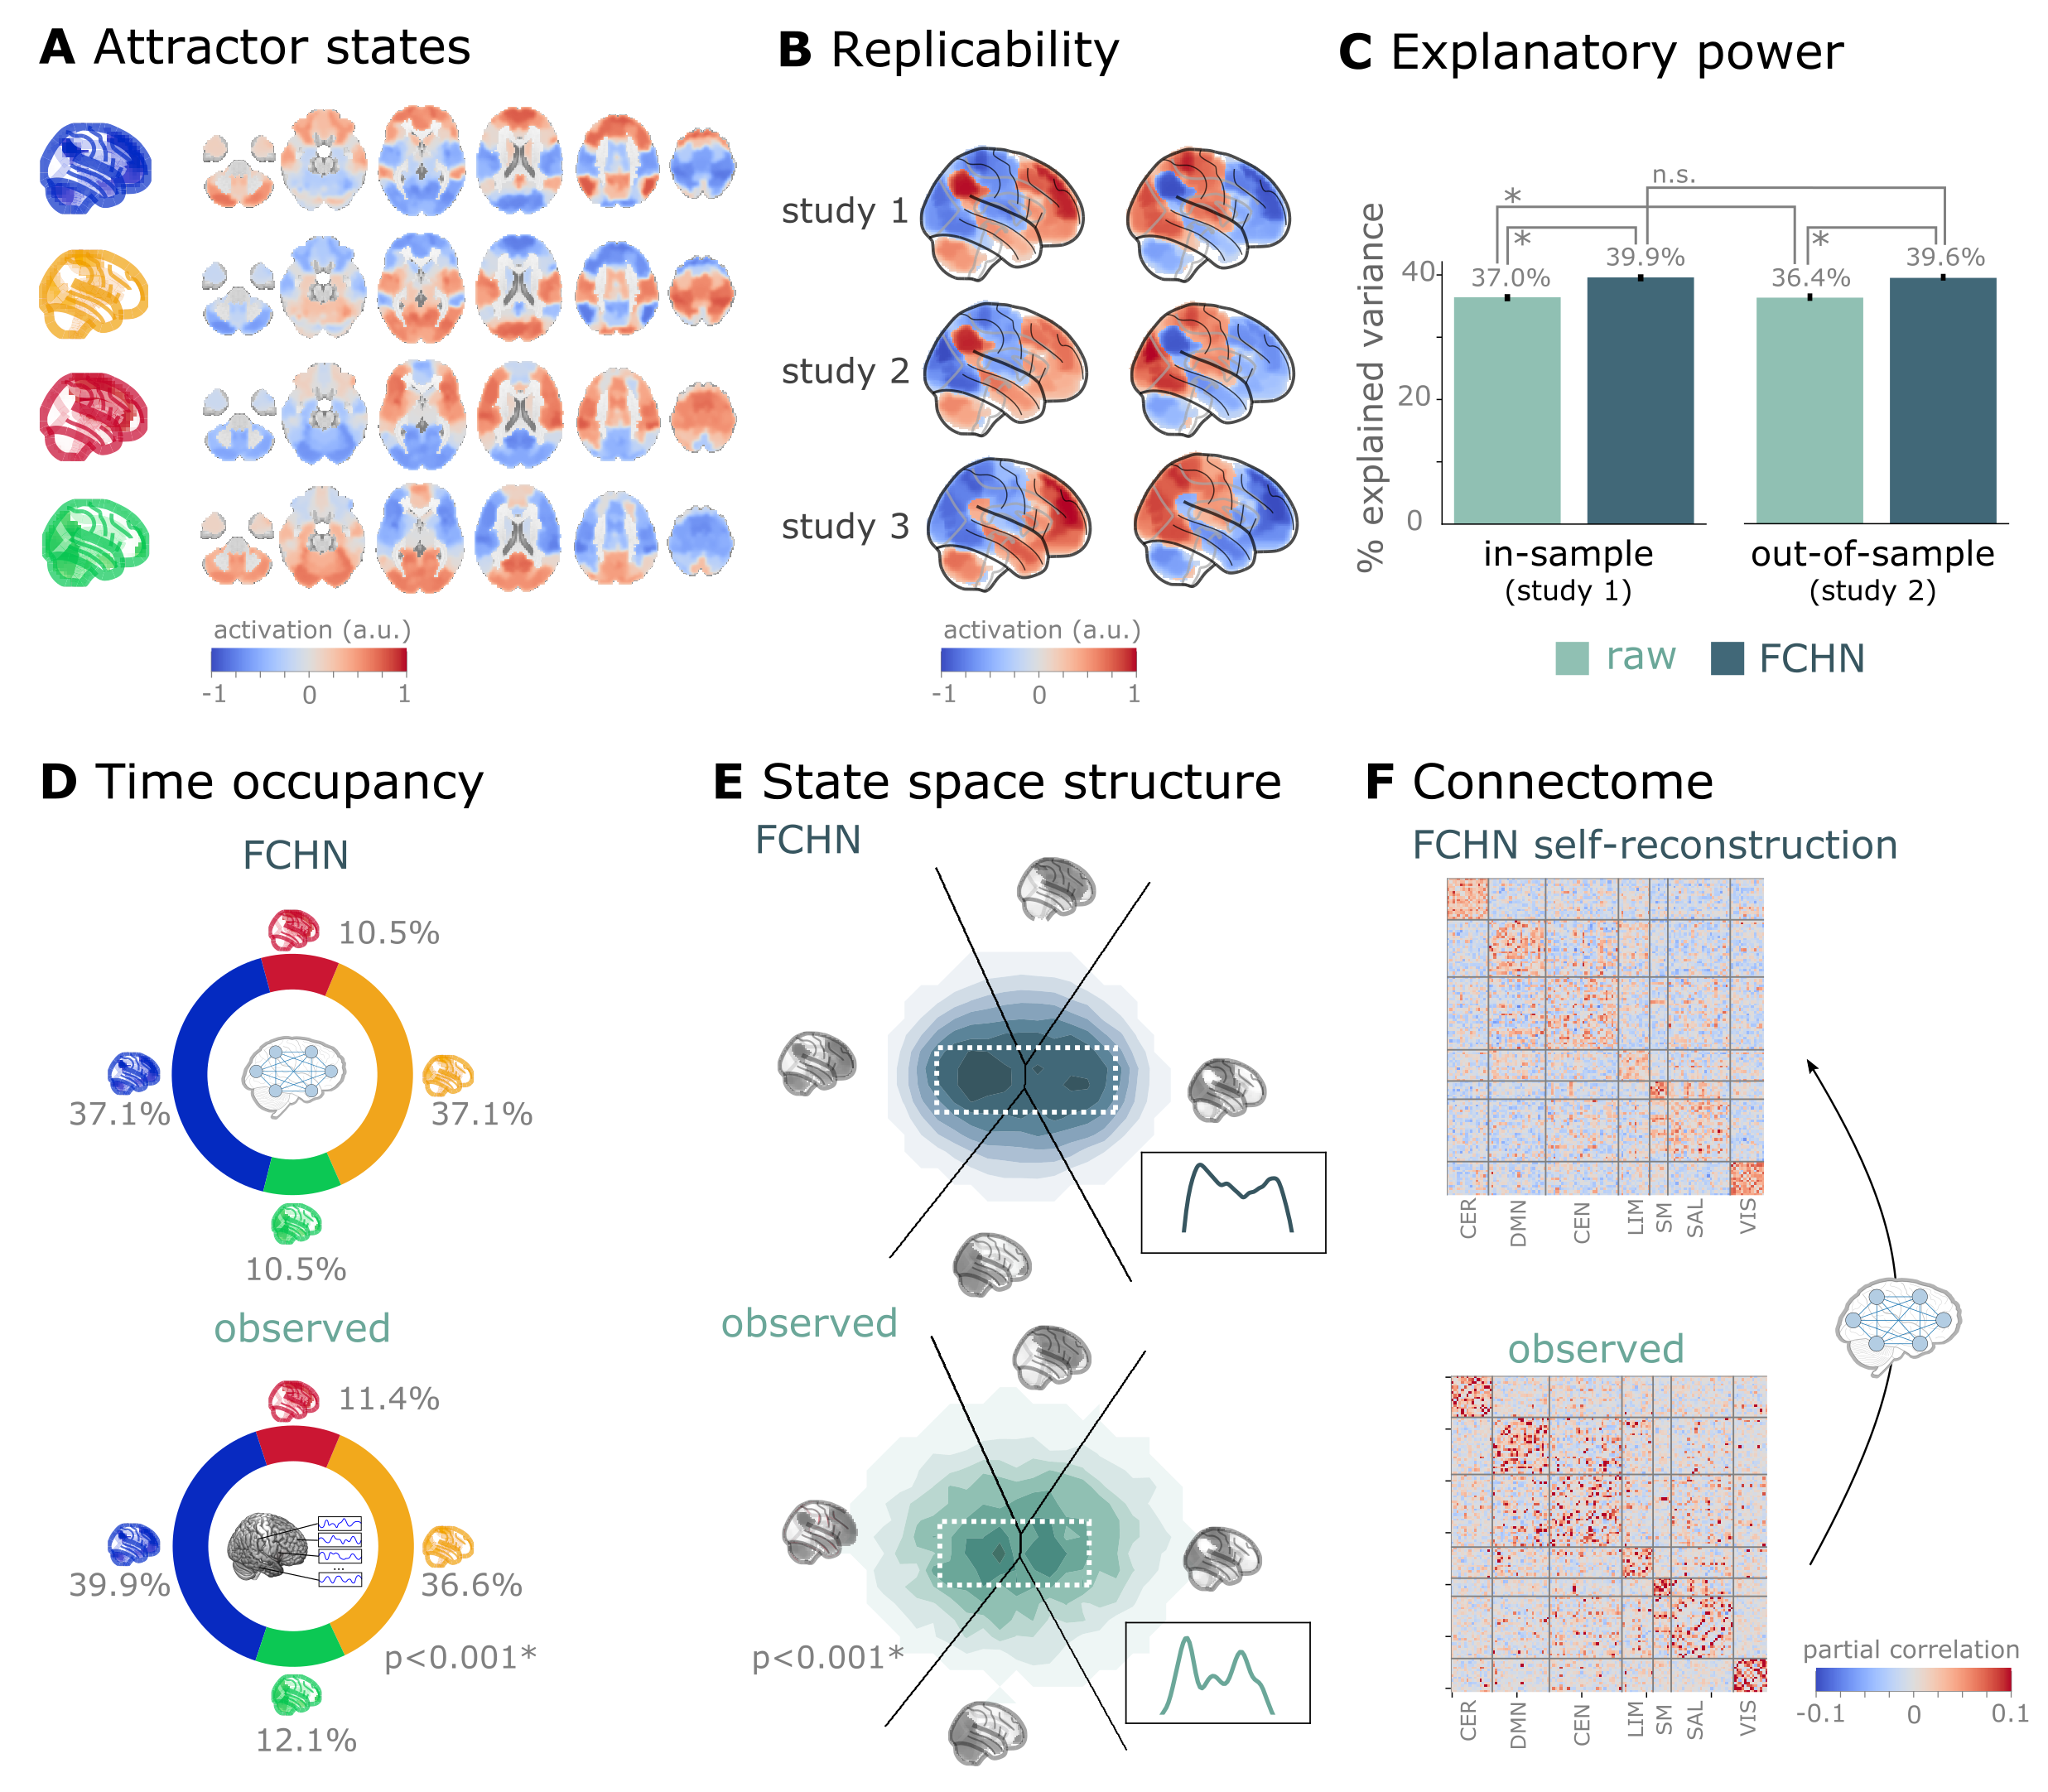
\includegraphics[width=0.7\linewidth]{files/face_validity-ddf49b1dc3ef72c114ec88cbbbdd5823.png}
\caption[]{\textbf{Connectome-based Hopfield networks reconstruct characteristics of real resting state brain activity.}\newline
\newline

\textbf{A} The four attractor states of the FCHN model from study 1 reflect brain activation
patterns with high neuroscientific relevance, representing sub-systems previously associated with 'internal context'
(blue), "external context" (yellow), "action/execution" (red) and "perception" (green)
\citep{golland2008data, cioli2014differences, chen2018human, fuster2004upper}.
\textbf{B} The attractor states show excellent replicability in two external datasets (study 2 and 3, mean correlation 0.93).
\textbf{C} The FCHN projection (first two PCs of the FCHN state space) explains significantly more variance (p\textless 0.0001) in the real
resting state fMRI data than principal components derived from the real resting state data itself and generalizes
better (p\textless 0.0001) to out-of-sample data (study 2). Error bars denote 99\% bootstrapped confidence intervals.
\textbf{D} The FCHN analysis accurately predicts (p\textless 0.0001) the fraction of time spent on the basis of the four attractor
states in real restring state fMRI data (study 1) and,
\textbf{E}, reconstructs the characteristic bimodal distribution of the real resting state data.
\textbf{F} Stochastic FCHNs are capable of self-reconstruction: the timeseries resulting from the stochastic relaxation procedure
mirror the co-variance structure of the functional connectome the FCHN model was initialized with.}
\label{rest-validity}
\end{figure}

Importantly, the discovered attractor states demonstrate a remarkable level of replicability (mean Pearson's
correlation 0.93) across the discovery datasets (study 1) and two independent replication datasets
(Table~\ref{tab-samples}, Figure~\ref{rest-validity}C).

Further analysis in study 1 showed that connectome-based Hopfield models accurately reconstructed multiple
characteristics of true resting-state data.

First, the FCHN projection accounted for a substantial amount of
variance in the real resting-state fMRI data in study 1 (mean $R^2=0.399$) and generalized well to out-of-sample data (study 2)
(mean $R^2=0.396$)  (Figure~\ref{rest-validity}E). Remarkably, the explained variance of the
FCHN projection significantly exceeded that of a PCA performed directly on the real resting-state fMRI data itself
($R^2=0.37$ and $0.364$ for in- and out-of-sample analyses).

Second, FCHN analyses accurately reconstruct true resting state brain state dynamics. During stochastic relaxation, the
FCHN model spends approximately three-quarters of the time on the basis of the first two attractor states, with an
equal distribution between them. The remaining one-quarter of the time is spent on the basis of the second pair of
attractor states, also equally distributed. To test whether we see similar state occupancy ratios in real resting state data,
we obtained normalized and cleaned mean timeseries in $m=122$ regions from all participants in study 1 and calculated
the attractor state of each time-frame via the FCHN model. We observed strikingly similar temporal occupancies to those
predicted by the model ($\Chi^2$-test with the null hypothesis of uniform occupancies: p\textless 0.00001,
Figure~\ref{rest-validity}B).

Third, FCHNs successfully reproduce fine-grained details of the bimodal distribution observed in the real resting-state fMRI data when projected onto the FCHN projection (Figure~\ref{rest-validity}F and Figure~\ref{attractors}E), suggesting that brain dynamics
are governed by a limited number of attractor states that emerge from the flow of activity across functional
connectivity networks.

Finally, during the stochastic relaxation procedure, FCHNs were found to generate regional time series that
preserve the covariance structure of the real functional connectome used for network initialization. This
important result indicates that a dynamic system in which activity flows across nodes of a complex network inevitably
"leaks" its underlying structure into the activity time series, providing a high level of construct validity for the
proposed approach (Figure~\ref{rest-validity}D).

It is important to reiterate that the proposed model was neither explicitly informed about, nor trained or optimized to reconstruct any of the investigated spatial (bi-modal distribution, explanatory performance) or temporal patterns (temporal state occupancy) of the brain.
The ability of the proposed connectome-based Hopfield model to reconstruct all these characteristics of real data strongly suggests that it captures essential relationships between the topology of the brain's functional connectome and the dynamics of its activation.

\subsubsection{An explanatory framework for task-based brain activity}\label{An explanatory framework for task-based brain activity}

The proposed framework offers a natural account for how activation patterns in the brain dynamically emerge form the
underlying functional connectivity. To illustrate this, we obtained task-based fMRI data from a study by
\citet{woo2015distinct} (Table~\ref{tab-samples}, n=33, see Figure~\ref{rest-validity}), investigating the neural
correlates of pain and its self-regulation. We found that time-frames obtained from periods with pain stimulation
(taking into account hemodynamics, see Methods for details) shoe a significantly different distribution on the FCHN projection
than time-frames obtained from periods without pain stimulation (permutation test for mean projection difference, p\textless 0.001, Figure~\ref{task-validity}A, left). Energies, as defined by the Hopfield model, were also significantly different between the two conditions
(permutation test, p\textless 0.001), with higher energies during pain stimulation.

When participants were instructed to up- or down-regulate their pain sensation (resulting in increased and decreased
pain reports and differential brain activity in the nucleus accumbens, NAc, (see \citep{woo2015distinct} for details)
we observed further changes of the location of momentary brain states on the Hopfield-projection (permutation test,
p\textless 0.001, Figure~\ref{task-validity}A, right). Interestingly, self-regulation did not manifest in significant energy changes
(permutation test, p=0.36).

\begin{figure}[!htbp]
\centering
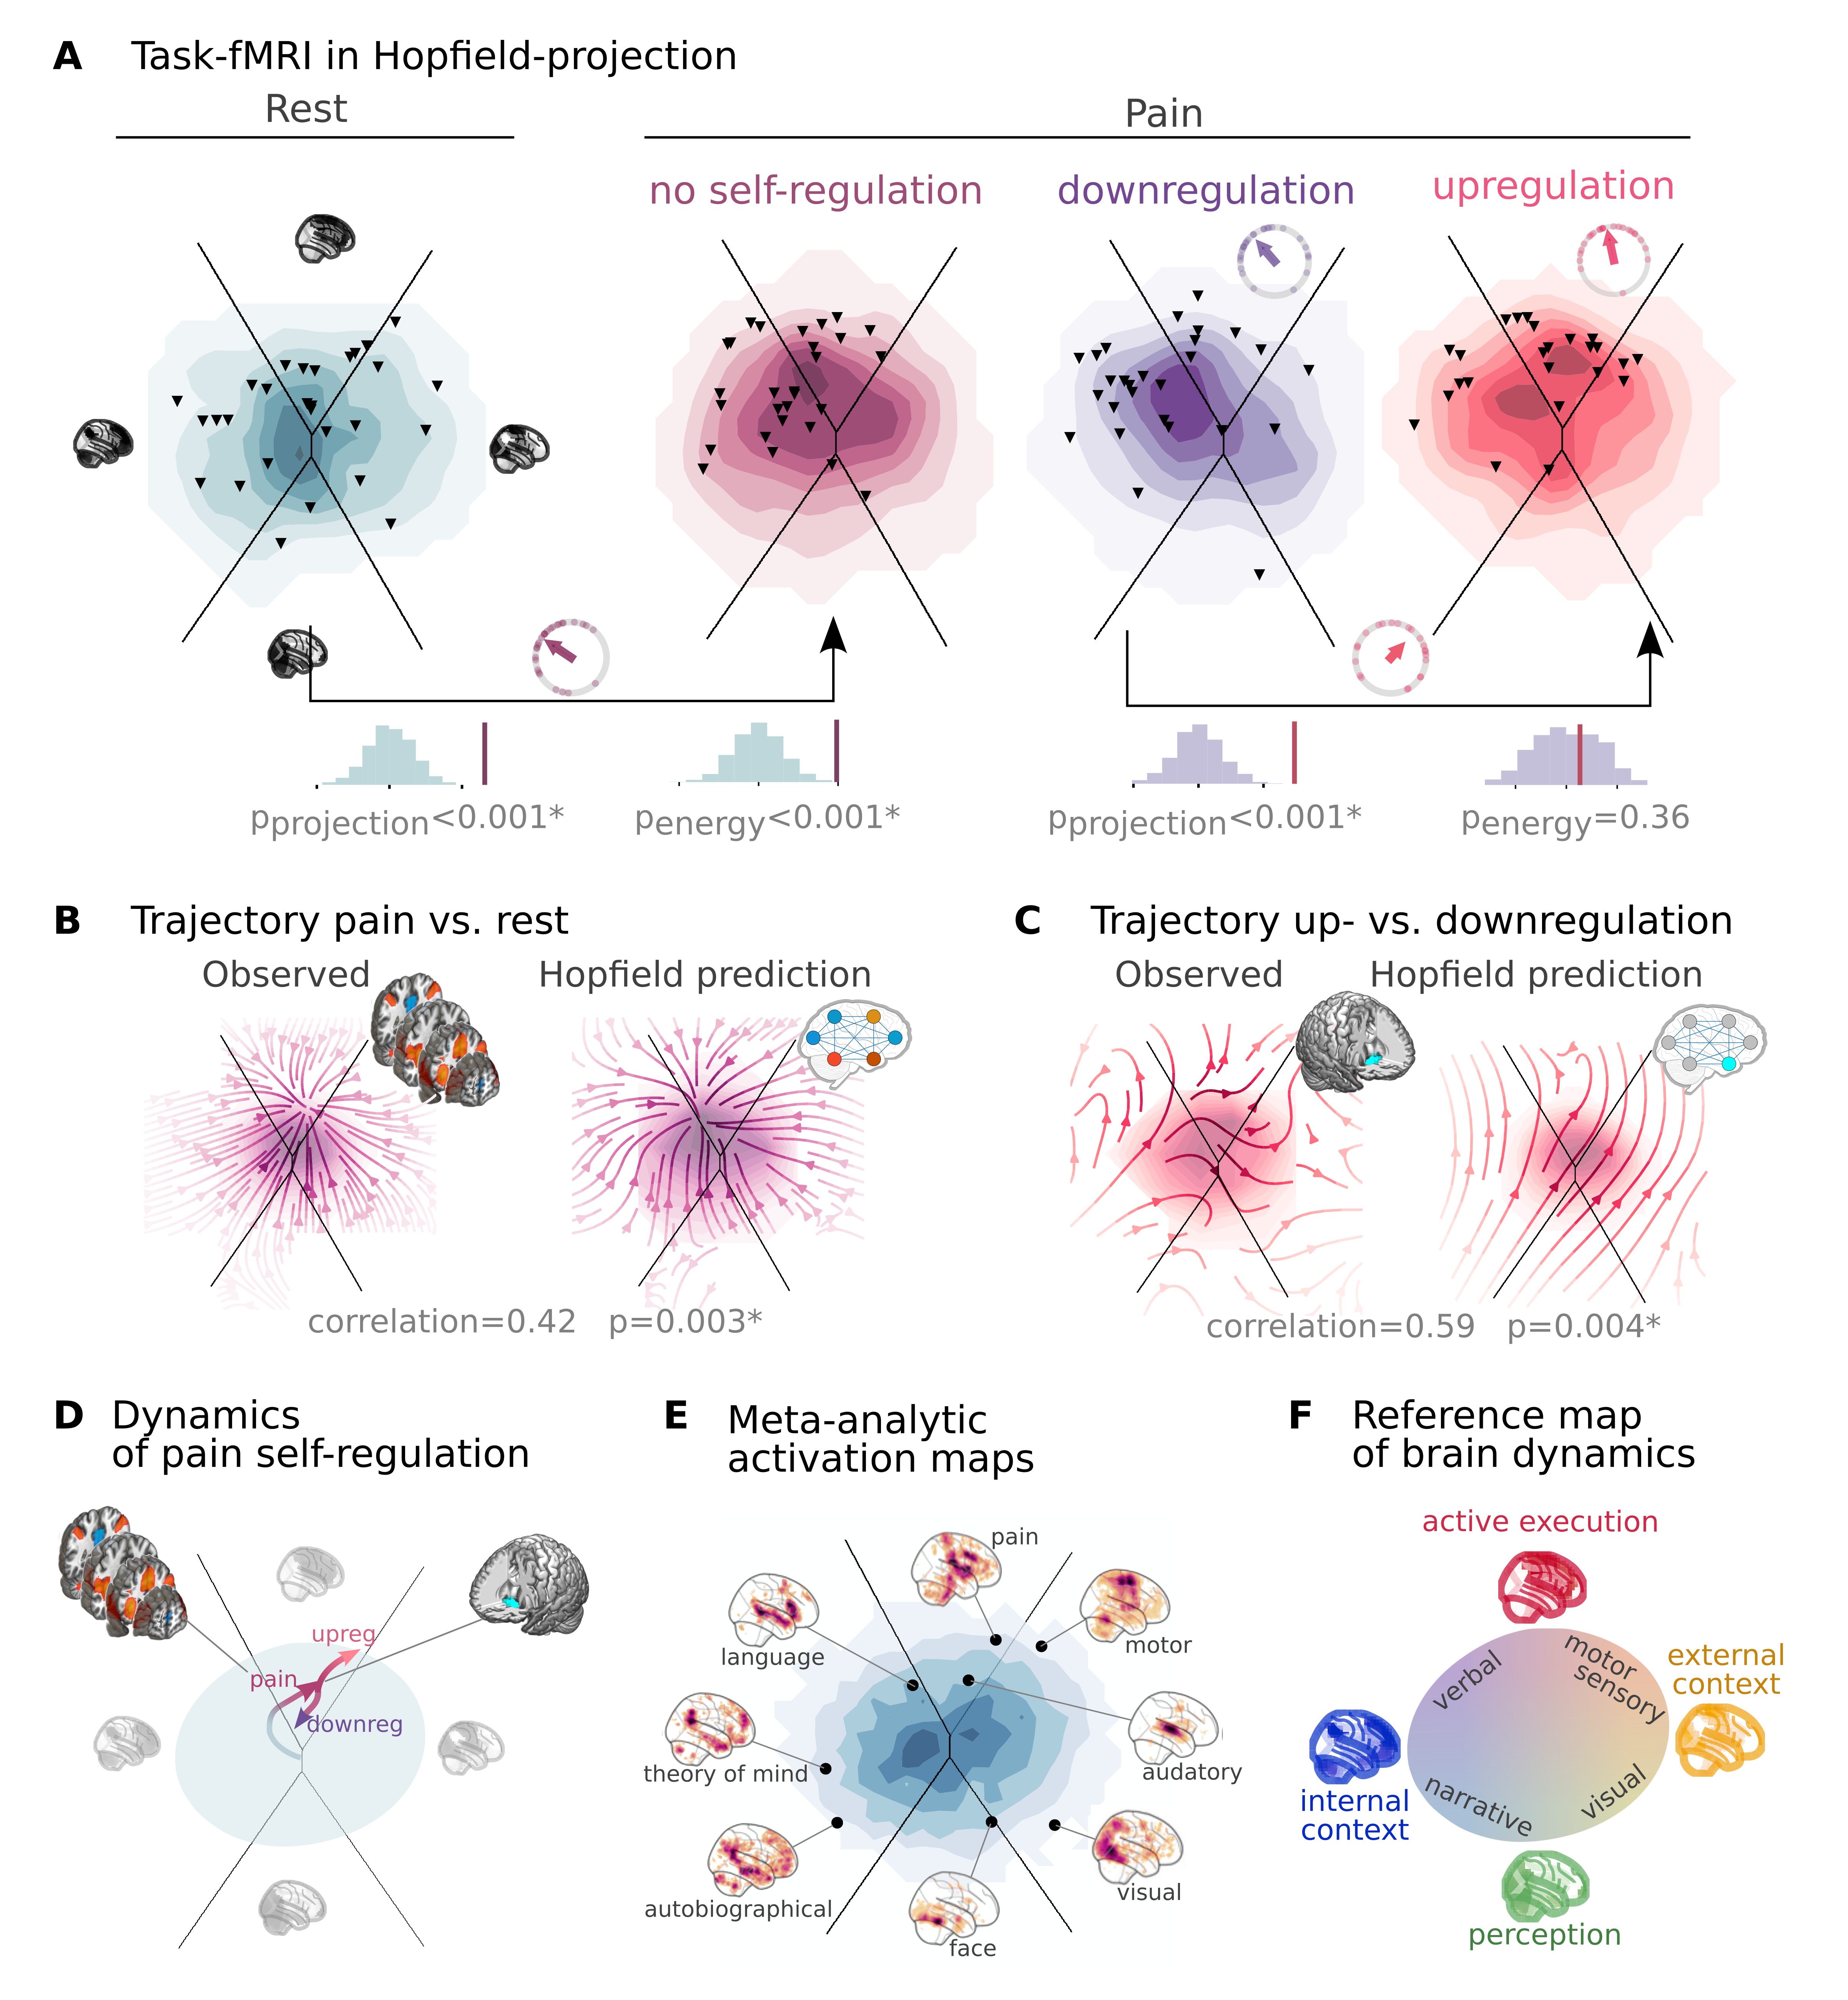
\includegraphics[width=0.7\linewidth]{files/task_validity-69351b40fd044cd5864d08d307a288ec.png}
\caption[]{\textbf{Empirical Hopfield-networks reconstruct real task-based brain activity.} \newline

\textbf{A} Functional MRI time-frames during pain stimulation from Table~\ref{tab-samples} (second FCHN projection plot)
and self-regulation (third and fourth) locate significantly differently on the FCHN projection than brain states
during rest (first projection, permutation test, p\textless 0.001 for all).  Energies, as defined by the Hopfield model, are also
significantly different between rest and the pain conditions (permutation test, p\textless 0.001), with higher energies during
pain stimulation. Triangles denote participant-level mean activations in the various blocks (corrected for
hemodynamics). Circle plots show the directions of the change for each individual (points) as well as the mean direction
across participants (arrow), as compared to the reference state (downregulation for the last circle plot, rest for all
other circle plots).
\textbf{B} Flow-analysis of the single time-frames (based on the vector pointing to the next time-frame)
reveal a non-linear difference in brain dynamics during pain and rest (left). When introducing weak
pain-related signal in the FCHN model during stochastic relaxation, it accurately reproduces these non-linear flow
differences (right).
\textbf{C} Simulating activity in the nucleus accumbens (NAc) (the region showing significant activity differences in \cite{woo2015distinct}) reconstructs the observed non-linear flow difference between up- and downregulation (left).
\textbf{D} Schematic representation of brain dynamics during pain and its up- and downregulation, visualized on the FCHN
projection. In the proposed framework, pain does not simply elicit a direct response in certain regions, but instead, shifts spontaneous brain dynamics towards the "action" subsystem, converging to a characteristic "ghost
attractor" of pain. Up-regulation by NAc de-activation exerts force towards a similar direction (thus increasing the probability of the emergence of "pain-activations") while down-regulation
by NAc activation exhibit an opposite effect on brain dynamics, leading to the brain less frequent "visiting"
pain-associated states.
\textbf{E} Visualizing meta-analytic activation maps on the FCHN projection captures intimate relations between the corresponding tasks and \textbf{F} serves as a basis for a FCHN-based theoretical interpretative framework for spontaneous and task-based brain dynamics. In the proposed framework, task-based activity is not a mere response to external stimuli in certain brain locations but a perturbation of the brain's characteristic dynamic trajectories, constrained by the underlying functional connectivity. From this perspective, "activity maps" from conventional task-based fMRI analyses capture time-averaged differences in these whole brain dynamics.}
\label{task-validity}
\end{figure}

These results provide an intuitive account for how the underlying functional connectivity of the brain can give rise to
different activation patterns, depending on the current (extrinsic or intrinsic) input. In the FCHN framework, change in
input (i.e. a task or stimulation) does not simply switch to the brain into a distinct "mode" of operation but acts as
a perturbation of the system's dynamics, resulting in mean activations changes that are only reliable measurable over
an extended period of time, as done by conventional task-based fMRI analyses.

The proposed framework offers much more than visualization and inference of resting state and task based data on the
FCHN projection. It provides a generative model for observed activity changes, enabling the prediction of brain
activity under different conditions. To illustrate this, we used the FCHN approach to simulate brain activity during pain
stimulation and self-regulation. First, we registered the frame-to-frame transitions (i.e. the vector on the 2-dimensional FCHN projection, pointing from a time-frame to the next one) in the real fMRI data for all four
conditions: rest, pain without self-regulation, downregulation, and upregulation.
Next, we evaluated the average direction in different segments of the projection plane, on a 6x6 grid. Finally, we
computed the difference between the mean directions observed during rest and pain (without regulation,
Figure~\ref{task-validity}B, left side), as well as between down- and upregulation (Figure~\ref{task-validity}C, left side).
This analysis unveiled non-linear trajectory patterns, indicating the most probable change in brain activity from a
given activity pattern, in a particular condition (pain without self-regulation or upregulation), as
compared to the reference state (rest and downregulation, respectively). In the case of pain versus rest, brain
activity tends to gravitate towards a distinct state, which we term the "ghost attractor" of pain (similar to \cite{vohryzek2020ghost}). In terms of attractor states, this belongs to the basin of the
attractor corresponding to action/execution. In case of up vs. downregulation, brain activity is pulled generally
towards a similar direction, but with a lack of a clear ghost attractor and, from most starting points, likely resulting in states that are closer to the pain-related "ghost attractor" point.

Next, our objective was to evaluate the extent to which the proposed framework can reconstruct the observed non-linear
dynamics. To simulate the alterations in brain dynamics during pain stimulation, we acquired a meta-analytic pain
activation map \citep{zunhammer2021meta} (n=603) and incorporated it as additional signal, along with Gaussian noise,
during the stochastic relaxation procedure. While incorporating such a signal naturally induces a minor linear shift
on the FCHN projection for each state generated during the stochastic relaxation procedure, this alone could not explain
the observed nonlinear dynamics in the real data (Supplementary material \textbf{X}). After conducting a
coarse-grained optimization across five different signal-to-noise (SNR) values (logarithmically spaced between
0.001 and 0.1), we found that by adding a minimal amount of signal (SNR = 0.01), the FCHN model achieved a remarkably
precise reconstruction of the observed non-linear disparities in brain dynamics between the pain and rest conditions,
including the characteristic pain-related "ghost attractor". (Spearman's $\rho$ = 0.42, p=0.003,
Figure~\ref{task-validity}B, right side).

The same model was also able to reconstruct the observed non-linear differences in brain dynamics between the up- and
downregulation conditions (Spearman's $\rho$ = 0.59, p=0.004) without any further optimization (SNR=0.01,
Figure~\ref{task-validity}C, right side). The only change we made to the model was the addition (downregulation) or
subtraction (upregulation) of activation in the NAc (the region in which \citep{woo2015distinct} observed significant
changes between up- and downregulation), with an SNR of 0.01.

These findings offer novel insights into the neural mechanisms underlying pain and its self-regulation, providing a
mechanistic explanation for the involvement of both nociception-related regions and the NAc (nucleus accumbens) in pain
regulation. (Figure~\ref{task-validity}D). Additionally, these findings emphasize that the conceptual differentiation
between resting and task states may, to a considerable extent, be an artificial dichotomy. Instead, even in the presence of highly salient
stimuli such as pain, the brain remains in a continuous state of flux, which is not radically altered by tasks and stimuli.

% -> discussion

To provide a comprehensive picture on how other tasks map onto the FCHN projection, we obtained various task-based
meta-analytic activation maps from Neurosynth (see Supplementary material X for details) and plotted them on the
FCHN projection (Figure~\ref{task-validity}E). This analysis reinforced and extended our interpretation of the four investigated attractor states and shed more light on how various functions are mapped on the axes of internal vs. external context and perception vs. action.
In this coordinate system of the FCHN projection, visual processing is labeled "external-perception", sensory-motor processes
"external-active", language, verbal cognition and working memory is labelled "internal-active" and long-term memory
as well as social and autobiographic narrative fall into the "internal-perception" regime (Figure~\ref{task-validity}F).

Together our results on task-based data highlight that the proposed generative framework can be used to simulate and predict brain dynamics under different conditions. Predicting the effect of lower or higher level of activity in certain regions (or lower or higher connectivity between them) on global brain dynamics and responses to various tasks provides unprecedented opportunities for forecasting the effect of interventions, such as pharmacological or non-invasive brain stimulation, on brain function.

\subsubsection{Clinical relevance}\label{Clinical relevance}

Computational models, such as the FCHN approach, have the potential to make a significant contribution to our mechanistic comprehension of various neurological and psychiatric disorders; which represents a crucial stride towards developing effective treatments. While providing a demonstration of the FCHN approach to yield such mechanistic insights in clinical populations is well outside the scope of the current study, here we present evidence that FCHN-based attractor state analysis can effectively capture and quantify several disease-related alterations in resting state brain dynamics.

For the sake of simplicity, we utilized one of the most simplistic FCHN-based analysis methods. Specifically, we applied the FCHN model from study 1 to allocate each time-frame of resting state data in the clinical samples (Table~\ref{tab-samples}) to one of the 4 attractor states. Then, we compared the average activity during resting state within each state across different clinical groups (with Bonferroni correction applied across brain regions and attractor states), resulting in a total of 122*4 comparisons per dataset. We analyzed three large public clinical databases as provided by the Autism Brain Imaging Data Exchange
(Table~\ref{tab-samples}: ABIDE, \citep{di2014autism}, the Centers of Biomedical Research Excellence
(Table~\ref{tab-samples}: COBRE, \citep{aine2017multimodal}) and the Alzheimer's Disease Neuroimaging Initiative
(Table~\ref{tab-samples}: ADNI, \citep{petersen2010alzheimer}).
In these analyses, resting state fMRI data of patients with autism spectrum disorder (ASD), schizophrenia (SCZ) and Alzheimer's disease
(AD) was contrasted to their respective control groups (typically developing controls for ASD, healthy control
participants for SCH and individuals with mild cognitive impairment (MCI) for AD, respectively).

\begin{figure}[!htbp]
\centering

\includegraphics[width=0.7\linewidth]{files/state_analysis-724b4260d15f0f95f34db1b82b5818f3.svg}
\caption[]{\textbf{Connectome-based Hopfield analysis as a sensitive tool for the study of clinical disorders.} \newline

We quantified attractor state activations in three clinical datasets (Table~\ref{tab-samples}) as the
individual-level mean activation of all time-frames belonging to the same attractor state. FCHN analyses of attractor
state activations revealed significant differences in all three datasets.
\textbf{A} Attractor state analysis of individuals with autism spectrum disorder (ASD) and typically developing controls (TD)
captures alterations similar to those previously associated to ASD-related perceptual atypicalities as well as atypical integration of information about the ``self'' and the ``other''.
\textbf{B} The most prominent Schizophrenia (SCZ)-related differences (as compared to healthy controls (HC) are related increased
activity of the internal subsystem and increased visual activations on the basis of the attractor state associated with perception.
\textbf{C} In Alzheimer's disease (AD), FCHN analysis revealed, among others, hyperactivity in the hippocampal formation (collateral sulcus) during perception, a commonly reported finding in AD.
and internal context (both of which together host long-term memory processes, see Figure~\ref{task-validity}F). All
results are corrected for multiple comparisons across brain regions and attractor states (122*4 comparisons)
with Bonferroni-correction. See Table~\ref{tab-clinical-results} Supplementary Table \textbf{X} for detailed results. \newline

\textit{\textbf{Abbreviations}: MCC: middle cingulate cortex, ACC: anterior cingulate cortex, pg: perigenual, PFC: prefrontal cortex, dm: dorsomedial, dl: dorsolateral, STG: superior temporal gyrus, MTG: middle temporal gyrus, ITG: inferior temporal gyrus, Caud/Acc: caudate-accumbens,  SM: sensorimotor, V1: primary visual, A1: primary auditory, Hipp: parahippocampal gyrus, Precun: precuneus, SMA: supplementary motor cortex, IPL: inferior parietal lobule, ASD: autism spectrum disorder, SCH: schizophrenia, AD: Alzheimer's disease.}}
\label{clinical-validity}
\end{figure}

We found several significant differences in the mean attractor activation of patients as compared to the respective
controls.

ASD (Figure~\ref{clinical-validity} left side) was found to be characterized by increased activity of the sensory-motor and middle cingular cortices during "action-execution" related states and increased visual and decreased sensory and auditory activity during "perception" states, likely reflecting the widely acknowledged, yet poorly understood, perceptual atypicalities in ASD \citep{hadad2019perception}.
ASD related changes in the internal-external axis were characterized by more involvement of the posterior cingulate, the precuneus, the nucleus accumbens, the dorsolateral prefrontal cortex (dlPFC), the cerebellum (Crus II and lobule VII) and inferior temporal regions during activity of the internalizing subsystem (Table \textbf{X}). While similar, default mode network (DMN)-related changes have often been attributed to an atypical integration of information about the ``self'' and the ``other'', a more detailed FCHN-analysis may help to further disentangle the specific nature of these changes.

In SCZ, the most prominent differences were found on the internal-external axis, with elevated activity in several brain regions during brain activity on the basin of the internal subsystem and decreased activity in the external subsystem. (Figure~\ref{clinical-validity}B, Table \textbf{X}). These findings are in line with the notion that, in schizophrenia, the forward projections have decreased functional connectivity relative to the back projections, and this may reduce the effects of external bottom-up inputs from the world relative to internal top-down thought processes \citep{rolls2021attractor}.
On the axis of the perception-action subsystems, the main difference was found in the visual and sensorimotor cortices, concordant with the widespread notion of visual and sensory deficits in SCZ \citep{javitt2009sensory, butler2008visual, adamek2022early}.

In the AD vs. MCI comparison, we found decreased resting state activations in several regions, including the inferior parietal lobule (IPL) and primary visual cortex, likely a consequence of high levels of amyloid-$\beta$ reducing synaptic excitatory transmission, resulting in synaptic failure and neuronal hypoactivity \citep{selkoe2002alzheimer}. A significant hyperactivity was found in the hippocampal formation (collateral sulcus) during perception states, which is
a commonly reported finding in AD \citep{aizenstein2015hippocampal, ewers2011neuroimaging}
(Figure~\ref{clinical-validity}C, \textbf{table}). Additionally, we observed increased activity in the supplementary motor cortex (SMA), a region known to exhibit minimal atrophy and hypometabolism in AD. This has been previously associated with the preservation of musical memories in AD \citep{jacobsen2015musical}.

\begin{table}
\centering
\caption[]{\textbf{The top ten largest activity changes in the three clinical studies.}  The attractor activity changes in ABIDE, COBRE and ADNI studies are presented in the order of their absolute effect size. All p-values are based on permutation tests and corrected for multiple comparisons. Attractor states are referred to with their index on Figure~\ref{clinical-validity}.}
\label{tab-clinical-results}
\begin{tabular}{p{\dimexpr 0.250\linewidth-2\tabcolsep}p{\dimexpr 0.250\linewidth-2\tabcolsep}p{\dimexpr 0.250\linewidth-2\tabcolsep}p{\dimexpr 0.250\linewidth-2\tabcolsep}}
\toprule
region & attractor & effect size & p-value \\
\hline
\textbf{autism spectrum disorder (ABIDE)} &  &  &  \\
primary auditory cortex & 1 & -0.126 & \textless 0.0001 \\
middle cingulate cortex & 0 & 0.109 & \textless 0.0001 \\
cerebellum lobule VIIb (medial part  ) & 3 & 0.104 & \textless 0.0001 \\
mediolateral sensorimotor cortex & 1 & -0.099 & 0.00976 \\
precuneus & 0 & 0.098 & \textless 0.0001 \\
middle superior temporal gyrus & 1 & -0.098 & \textless 0.0001 \\
frontal eye field & 1 & -0.095 & \textless 0.0001 \\
dorsolateral sensorimotor cortex & 1 & -0.094 & 0.00976 \\
posterior cingulate cortex & 0 & 0.092 & \textless 0.0001 \\
dorsolateral prefrontal cortex & 2 & -0.092 & \textless 0.0001 \\
\textbf{schizophrenia (COBRE)} &  &  &  \\
angular gyrus & 1 & -0.139 & \textless 0.0001 \\
mediodorsal visual cortex & 1 & 0.138 & \textless 0.0001 \\
superior parietal lobule & 0 & 0.128 & \textless 0.0001 \\
mediodorsal visual cortex (posterior part) & 0 & -0.119 & \textless 0.0001 \\
posterior visual cortex (dorsomedial part) & 1 & 0.114 & 0.00976 \\
anterior middle frontal gyrus & 2 & -0.105 & \textless 0.0001 \\
dorsomedial prefrontal cortex & 2 & -0.102 & \textless 0.0001 \\
posterior cingulate cortex & 3 & 0.102 & \textless 0.0001 \\
dorsolateral prefrontal cortex & 3 & 0.101 & \textless 0.0001 \\
medial orbital gyrus & 3 & 0.099 & \textless 0.0001 \\
\textbf{Alzheimer's disease (ADNI)} &  &  &  \\
cerebellum lobule IX (middle part) & 0 & -0.154 & 0.00976 \\
parahippocampal gyrus & 1 & 0.139 & \textless 0.0001 \\
cerebellum lobule IX (dorsal part) & 1 & 0.132 & 0.02928 \\
medial visual cortex (posterior part) & 0 & -0.129 & \textless 0.0001 \\
occipitoparietal association area (ventral part) & 0 & -0.128 & 0.00976 \\
ventral visual cortex (medial part) & 0 & -0.124 & 0.02928 \\
left inferior parietal lobule & 2 & -0.11 & \textless 0.0001 \\
right inferior parietal lobule & 2 & -0.095 & \textless 0.0001 \\
left cerebellar crusII (posterior part) & 2 & -0.094 & \textless 0.0001 \\
anteromedial somatosensory cortex & 2 & 0.093 & \textless 0.0001 \\
\bottomrule
\end{tabular}
\end{table}

\subsection{Discussion}\label{Discussion}

Regions of the brain are in a constant flux of information exchange, giving rise to characteristic co-activations patterns.
The degree to which activation in a region triggers activation in another is different for every pair of regions, spanning an
intricate network, commonly referred to as the functional connectome.

In this study, we have introduced a simple yet robust framework that elucidates how activity propagation within the functional connectome orchestrates large-scale brain dynamics, leading to distinct brain states accompanied by characteristic dynamic responses to perturbations.
Through a series of experiments, we have demonstrated that the proposed model can effectively reconstruct and predict large-scale brain dynamics across diverse conditions.

The presented approach offers a fresh perspective on large scale brain dynamics and offers unparalleled prospects for forecasting the impact of interventions, including pharmacological treatments or non-invasive brain stimulation, on brain function.

The construct validity of our model is rooted in the activity flow principle, first introduced by
\citet{cole2016activity}. The activity flow principle states that activity in a brain region can be predicted by a weighted combination of the activity of all other regions, where the weights are set to the functional connectivity of those regions to the held-out region. This principle has been shown to hold across a wide range of experimental and clinical conditions
\citep{cole2016activity, ito2017cognitive, mill2022network, hearne2021activity, chen2018human}.

\begin{quote}
ToDo: latent FC-based modelling: \cite{McCormick_2022}
\end{quote}

Our model was born from the intuition that the repeated, iterative application of the activity flow equation in a system that exhibits close analogies with a type of recurrent artificial neural network known as Hopfield networks
\citep{hopfield1982neural}.

Hopfield networks have previously been shown to exhibit a series of characteristics that are also highly relevant for
brain function, including the ability to store and recall memories \citep{hopfield1982neural}, self-repair \citep{murre2003selfreparing},
a staggering robustness to noisy or corrupted inputs \citep{hertz1991introduction} and the ability to produce
multistable dynamics organized by the "gravitational pull" of a finite number of attractor states
\citep{khona2022attractor}. While many of such properties of Hopfield networks have previously been proposed as a model for micro-scale neural systems (see \cite{khona2022attractor} for a review), the proposed link between macro-scale activity propagation and Hopfield networks allows transferring the vast body of knowledge on Hopfield networks to the study of large-scale brain dynamics.

Integrating Cole's activity flow principle with the Hopfield neural network architecture mandates the initiation of network weights with functional connectivity values, specifically partial correlations as suggested by \citet{cole2016activity}.
Considering the functional connectome as weights of an already trained neural network distinguishes our methodology not only from conventional computational modeling strategies, which usually rely on the structural connectome as a proxy for polysynaptic connectivity \citep{cabral2017functional}, but also from "neuroconnectionist" approaches that employ explicit training procedures \citep{doerig2023neuroconnectionist}.
Functional connectome-based Hopfield neural network (FCHN) models can be conceptualized as a streamlined alternative to those methodologies, offering significant advantages.

First, the intricate nature of conventional computational models of the brain leads to an exponential proliferation of the parameter space.
While finely detailed computational models hold promise for providing comprehensive insights, they are prone to overfitting real data \citep{breakspear2017dynamic}.
In contrast to those approaches, the basic form of the FCHN approach comprises solely two hyperparameters (temperature and noise) and yields notably consistent outcomes across an extensive range of these parameter. To underscore the potency of this simplicity and stability, in the present work, we intentionally minimized the fine-tuning of these parameters. We fixed the temperature parameter at a value that robustly provides 4 attractor
states and used a single noise level for all experiments (selected with a coarse optimization procedure to approximately
mimic the distribution of real data).

Second, high model complexity usually translates to a greater challenge in terms of interpretability.
The FCHN approach offers straightforward interpretations, as it establishes a
direct link between two highly prevalent metrics of brain function: functional connectivity and brain activity.
This connection is not solely conceptual, but also mathematical, facilitating the exploration and prediction of alterations in the system's dynamics in response to perturbations affecting both activity and connectivity.

Given its simplicity, it is remarkable, if not surprising, how accurately the FCHN model is able to
reconstruct and predict brain dynamics under a wide range of conditions. Particularly surprising is the result
that the 2-dimensional FCHN projection can explain more variance in real resting state fMRI data than the first two principal components derived from the data itself.
Here we propose that the explanation for the extraordinary performance of the FCHN model in reconstructing brain function is that it captures essential principles of the underlying dynamics that can be used to reconstruct the brain's activation state-space even if our empirical measurements are corrupted by noise and low sampling rate.

The known noise-tolerance of the proposed architecture may also explain the high replicability of FCHN attractors across different
datasets (study 2 and 3). The observed level of replicability allowed us to re-use the FCHN model constructed with the
connectome of study 1 for all subsequent studies (2-8), without any further fine-tuning or study-specific parameter
optimization of the FCHN model.

Attractor states are a key concept in the FCHN framework. They are not only local minima in the state-space but act as a driving force for the dynamic trajectories of brain activity. Nevertheless, attractor states should not be confused with the conventional notion of brain states (e.g. co-activation patterns \citep{chen2015introducing}). In the FCHN framework, attractor states can rather be conceptualized as "Platonic idealizations" of brain activity, that are continuously approximated - but never reached - by the brain, resulting in a complex, clustered distribution of actual brain activation patterns. In or notion, this clusteredness is what gives rise to the commonly described reoccurring quasi-periodic patterns, commonly referred to as brain states.

Relying on previous work, we can establish a relatively straightforward (yet somewhat speculative) mapping between attractor states and brain function. We refer to the first two attractor states as the internal and external subsystems \citep{golland2008data, cioli2014differences}. Both FCHN-reconstructed and empirical brain activity spans the highest variance along the axis corresponding to this attractor state pair, suggesting that the robust and widely described observation of the brain state we commonly refer to as the DMN is a consequence of the brain's tendency to commute between the two state-space clusters emerging along this primary axis.
The third and fourth attractor states accurately map to the previously described perception-execution axis within the brain \citep{fuster2004upper}. The four investigated attractor states display an appealing correspondence to recent theories of brain function that capitalize on Friston's free energy principle \citep{friston2006free} and postulate the necessary existence of subsystems for active and perceptual inference \citep{friston2023free} as well as a hierarchically organized (i.e. external and internal) subsystems that give rise to consciousness \citep{ramstead2023inner}.

In the FCHN framework, the brain is in a constant state of flux, traversing extended areas of the state space. Task-based brain activity in this framework is not a mere response to external stimuli in certain brain locations but a perturbation of the brain's characteristic dynamic trajectories, shifting towards the realms of those attractor states that represent the type of function required by the task or stimuli. In other words brain activity is only perturbed by external input, rather than predestined. We exemplified this with the case of the self-regulation of pain (study 4).
In our analyses, the FCHN approach was not only able to capture participant-level activity changes induced by pain and its self-regulation (showing significant differences on the FCHN projection and in terms of state energy), but also accurately predicted the non-linear changes in activity flow induced by characteristic activity changes and give a mechanistic account for how activity change in a single region (NAcc) may result in a significantly altered pain experience.

Brain dynamics can not only be perturbed by task or other types of experimental or naturalistic interventions, but also
by pathological alterations. In our analysis of clinical samples (studies 6-8), we found that FCHN-based analysis of mean attractor activations is a highly sensitive tool to characterize neural correlates of autism spectrum disorder (ASD), Schizophrenia (SCH) and Alzheimer's disease (AD), even with the most conservative correction for multiple comparisons. These results - although descriptive in their nature - provide a proof-of-concept regarding the clinical potential of the proposed approach and pave the way for more elaborate applications of the FCHN approach in clinical and translational research.

Together, our findings open up a series of exciting opportunities for the mechanistic understanding of brain function.

First, the 2-dimensional FCHN projection offers a common framework for the interpretations of any brain activity patterns, and conceptualize changes related to various behavioral or clinical states or traits as a shift in brain dynamics along the axes determined by the attractor states.

Second, the FCHN model's utility extends far beyond the sole detection of such altered brain dynamics. By its generative nature, FCHN analyses may provide insights into the causes of changes in brain dynamics, by for instance, identifying the regions or connections that act as an Achilles heel in generating such changes. Such analyses could, for instance, aid the differentiation of primary causes and secondary effects of particular activity or connectivity changes in various clinical conditions.

Third, the FCHN approach might provide testable predictions about the effects of interventions on brain functions,
like pharmacological or non-invasive brain stimulation (e.g. transcranial magnetic or direct current stimulation,
focused ultrasound) or neurofeedback. Obtaining such predictions on the individual level (e.g. based on the individual functional connectome) might aid the design of personalized medicine approaches.

In this initial work, we presented the simplest possible implementation of the FCHN concept. It is clear that the presented analyses   exploit only a small proportion of the richness of the full state-space dynamics reconstructed by the FCHN model.
There are many potential way to further improve the utility of the FCHN approach. Increasing the number of reconstructed attractor states (by increasing the temperature parameter), investigating higher-dimensional dynamics, fine-tuned hyperparameters, the effect of
different initializations and perturbations are all important direction for future work, with the potential to further
improve the model's accuracy and usefulness.

\begin{quote}
\textbf{other potential topics}:

\begin{itemize}
\item why no HRF modelling (could be a possible extension, but it is also not part of the activity flow approach and we don't reconstruct time series, but rather activations)
\item is the connectome stationary? See arguments by the Cole-group.
\item why rs-fMRI connectome (could be latent-FC a'la McCormick, 2022)
\item the FCHN model is not a model of brain function, but a model of brain dynamics. It does not strive to explain various brain regions ability to perform certain computations, but the brain's characteristic trajectories, which are perturbed by tasks and other types of interventions.
\end{itemize}
\end{quote}

\subsection{Conclusion}\label{Conclusion}

To conclude, here we have proposed a lightweight, high-level computational framework that accurately captures and predicts brain dynamics
under a wide range of conditions. The framework models large-scale activity flow in the brain with a recurrent
artificial neural network architecture that, instead of being trained to solve specific tasks or mimic certain dynamics,
is simply initialized with the empirical functional connectome. The framework identifies neurobiologically meaningful
attractor states and provides a model for how these restrict brain dynamics. The proposed framework, referred to as the
connectome-based Hopfield neural network (FCHN) model, can accurately reconstruct and predict brain dynamics under a wide range of
conditions, including resting state, task-induced activity changes, as well as in various brain disorders. FCHNs establish a conceptual link between connectivity and activity provide and offer a simple, robust, and highly interpretable computational alternative to the conventional descriptive approaches to investigating brain function. The generative nature of the proposed model opens up a series of exciting opportunities for future research, including novel ways of assessing causality and mechanistic understanding, and the possibility to predict the effects of various interventions, thereby paving the way for novel personalized medical approaches.

\subsection{Methods}\label{Methods}

\subsubsection{Data}\label{Data}

We obtained functional MRI data from 7 different sources (Table~\ref{tab-samples}).
We included three resting state studies with healthy volunteers (study 1, study 2, study 3), one task-based study (study 4), 8 meta-analytic task-based activation patterns obtained from Neurosynth (study 5), and three additional resting state studies focusing on specific disease conditions. These include the ABIDE (Autism Brain Imaging Data Exchange) study on Autism Spectrum Disorder (ASD, study 6, \cite{di2014autism}), the COBRE (Center for Biomedical Research Excellence) study on Schizophrenia (study 8, \citep{aine2017multimodal}) and data obtained from ADNI (Alzheimer's Disease Neuroimaging Initiative database (\href{http://adni.loni.usc.edu}{adni.loni.usc.edu}) on Alzheimer's Disease (study 7, \citep{petersen2010alzheimer}).

\begin{table}
\centering
\caption[]{\textbf{Datasets and studies.} The table includes details about the study modality, analysis, sample size, mean age, gender distribution, and references.}
\label{tab-samples}
\begin{tabular}{p{\dimexpr 0.143\linewidth-2\tabcolsep}p{\dimexpr 0.143\linewidth-2\tabcolsep}p{\dimexpr 0.143\linewidth-2\tabcolsep}p{\dimexpr 0.143\linewidth-2\tabcolsep}p{\dimexpr 0.143\linewidth-2\tabcolsep}p{\dimexpr 0.143\linewidth-2\tabcolsep}p{\dimexpr 0.143\linewidth-2\tabcolsep}}
\toprule
study & modality & analysis & n & age (mean$\pm$sd) & \%female & references \\
\hline
study 1 & resting state & discovery & 41 & 26.1$\pm$3.9 & 37\% & \cite{Spisak_2020} \\
study 2 & resting state & replication & 48 & 24.9$\pm$3.5 & 54\% & \cite{Spisak_2020} \\
study 3 & resting state & replication & 29 & 24.8$\pm$3.1 & 53\% & \cite{Spisak_2020} \\
study 4 & task-based & pain self-regulation & 33 & 27.9 $\pm$ 9.0 & 66\% & \cite{Woo_2015} \\
study 5 (Neurosynth) & task-based & coordinate-based meta-analyses & 14371 studies in total & \textbullet~~\newline
 & \textbullet~~\newline
 & \cite{Tor_D__2011} \\
study 6 (ABIDE, NYU sample) & resting state & Autism Spectrum Disorder & ASD: 98, NC: 74 & 15.3$\pm$6.6 & 20.9\% & \citep{di2014autism} \\
study 7 (COBRE) & resting state & Schizophrenia & SCH: 60, HC: 72 & 37.0$\pm$12.6 & 29.4 \% & \citep{aine2017multimodal} \\
study 8 (ADNI) & resting state & Alzheimer's Disease vs. Mild Cognitive Impairment & AD: 34, MCI 99: & 72.5$\pm$7.5 & 50.4\% & \citep{petersen2010alzheimer} \\
\bottomrule
\end{tabular}
\end{table}

Study 1 (n=41) was used to evaluate the ability of the proposed approach to reconstruct resting state brain activity. Study 2 and 3 (n = 48 and 29, respectively) served es replications studies for these analyses. Further details on study 1-3 are described in \cite{Spisak_2020}. The ability of the proposed approach to model task-based perturbation of brain dynamics was evaluated in Study 4, which consisted of 8 runs of nine task-based fMRI runs for each of the 33 healthy volunteers. In all runs, participants received heat pain stimulation. Each stimulus lasted 12.5 seconds, with 3-second ramp-up and 2-second ramp-down periods and 7.5 seconds at target temperature. Six levels of temperature were administered to the participants (level 1: 44.3°C; level 2: 45.3°C; level 3: 46.3°C; level 4: 47.3°C; level 5: 48.3°C; level 6: 49.3°C). In this analysis we used run 1 (passive experience)  run 3 (down-regulation) and run 7 (up-regulation). Participants were asked to cognitively ``increase'' (regulate-up) or ``decrease'' (regulate-down) pain intensity. See \citet{woo2015distinct} for details.
To obtain fMRI activation maps for tasks other than pain, we used Neurosynth(\cite{Tor_D__2011}), a web-based platform for large-scale, automated synthesis of functional magnetic resonance imaging (fMRI) data. We performed 8 different coordinate-based meta-analyses with the terms "motor", "auditory", "visual", "face", "autobiographical", "theory mind", "language" and "pain" and obtained the z-scores maps from a two-way ANOVA, comparing the coordinates reported for studies with and without the term of interest, and testing for the presence of a non-zero association between term use and voxel activation. The meta-analyses encompassed a total  of 14371 different studies.

In study 6 and 7 (ABIDE, COBRE respectively), we obtained preprocessed regional timeseries data from the Preprocessed Connectome Project \citep{craddock2013towards}, as shared (\href{https://osf.io/hc4md}{https://osf.io/hc4md}) by \citet{dadi2019benchmarking}. Preprocessed regional timeseries data for study 8 (ADNI) was obtained from from the Alzheimer's Disease Neuroimaging Initiative database (\href{http://adni.loni.usc.edu}{adni.loni.usc.edu}). All preprocessed timeseries data were obtaoined with the 122-region version of the BASC (Bootstrap Analysis of Stable Clusters) brain atlas \citep{bellec2010multi}.

\subsubsection{Preprocessing and timeseries extractions}\label{Preprocessing and timeseries extractions}

Functional MRI data from studies 1-4 was preprocessed with our in-house analysis pipeline, called the RPN-pipeline (\href{https://github.com/spisakt/RPN-signature}{https://github.com/spisakt/RPN-signature}). The RPN-pipeline is based on PUMI (Neuroimaging Pipelines Using Modular workflow Integration, \href{https://github.com/pni-lab/PUMI}{https://github.com/pni-lab/PUMI}), a nipype-based \citep{gorgolewski2011nipype} workflow management system. It capitalizes on tools from FSL \citep{jenkinson2012fsl}, ANTS \citep{avants2011reproducible} and AFNI \citep{cox1996afni}, with code partially adapted from the software tools C-PAC \citep{craddock2013towards} and niworkflows \citep{esteban2019fmriprep}, as well as in-house python routines. We run the containerized version of the pipeline with default parameters, as in \cite{Spisak_2020}.

Brain extraction from both the anatomical and the structural images, as well, as tissue-segmentation from the anatomical images was performed with FSL bet and fast64. Anatomical images were linearly and non-linearly co-registered to the 1mm-resolution MNI152 standard brain template brain with ANTs (see \href{https://gist.github.com/spisakt/0caa7ec4bc18d3ed736d3a4e49da7415}{https://gist.github.com/spisakt/0caa7ec4bc18d3ed736d3a4e49da7415} for source code).

Functional images were co-registered to the anatomical images with the boundary-based registration technique of FSL flirt. All resulting transformations were saved for further use. The preprocessing of functional images happened in the native image space, without resampling. Realignment-based motion-correction was performed with FSL mcflirt. The resulting six head motion estimates (3 rotations, 3 translations), their squared versions, their derivates and the squared derivates (known as the Friston-24-expansion, \cite{friston1996movement}) was calculated and saved for nuisance correction. Additionally, head motion was summarized as framewise displacement (FD) timeseries, according to Power's method \citep{power2012spurious}, to be used in data censoring and exclusion. After motion-correction, outliers (e.g. motion spikes) in timeseries data were attenuated using AFNI despike. The union of the eroded white-matter maps and ventricle masks were transformed to the native functional space and used for extracting noise-signal for anatomical CompCor correction \citep{behzadi2007component}.

In a nuisance regression step, 6 CompCor parameters (the 6 first principal components of the noise-region timeseries), the Friston-24 motion parameters and the linear trend were removed from the timeseries data with a general linear model. On the residual data, temporal bandpass filtering was performed with AFNI's 3DBandpass to retain the 0.008--0.08\,Hz frequency band. To further attenuate the impact of motion artifacts, potentially motion-contaminated time-frames, defined by a conservative FD\,\textgreater \,0.15\,mm threshold, were dropped from the data (known as scrubbing, \cite{satterthwaite2013improved}). Participants were excluded from further analysis if more then 50\% of frames were scrubbed.

The 122-parcel version of the BASC multi-resolution functional brain atlas \citep{bellec2010multi} was individualized; it was transformed to the native functional space of each participant and masked by the  grey-matter mask obtained from the anatomical image, to retain grey-matter voxels only. Voxel-timeseries were averaged over these individualized BASC regions.

\subsubsection{Functional connectome}\label{Functional connectome}

Regional timeseries were ordered into large-scale functional modules (defined by the 7-parcel level of the BASC atlas) for visualization purposes.
Next, in all datasets, we estimated study-level mean connectivity matrices by regularized partial correlation, via the Graphical Lasso algorithm that estimates a sparse precision matrix by solving a Lasso problem and an L1 penalty for sparsity, as implemented in nilearn \citep{abraham2014machine}. Diagonal elements of the matrices were set to zero.

\subsubsection{Connectome-based Hopfield networks}\label{Connectome-based Hopfield networks}

Hopfield networks, a type of artificial neural network, consist of a single layer of $m$ fully connected nodes \citep{hopfield1982neural}, with activations $\bold{a} = (a_1, \dots, a_m )$. Hopfield networks assign an energy to any arbitrary activity configurations:

\begin{equation}
\label{energy-function}
E = - \frac{1}{2}  \bold{a}^{T} \bold{W} \bold{a} + \bold{a}^{T}\bold{b}
\end{equation}

where $W$ is the weight matrix with element w\_\{i,j\} denoting the weight between nodes i and j and $\bold{b}$ is the bias, which is set to $\bold{b} = 0$ for all experiments.

During the so-called relaxation process, the activities of the nodes are iteratively updated until the network converges to a stable state, known as an attractor state. The dynamics of the network are governed by the equation referenced as eq (\ref{hopfield-update}), or in matrix form:

\begin{equation}
\label{hopfield-update-matrix}
\dot{\bold{a}} = S(\beta \bold{W} \bold{a} - \bold{b})
\end{equation}

where $\dot{\bold{a}} = (\dot{a}_1, \dots, \dot{a}_m)$ is the activity in the next iteration and $S(.)$ is the sigmoidal activation function ($S(a) = tanh(a)$ in our implementation) and $\beta$ is the temperature parameter.
During the stochastic relaxation procedure, we add weak Gaussian noise to each node's activity at every iteration:

\begin{equation}
\label{hopfield-update-matrix-stochastic}
\dot{\bold{a}} = S(\beta \bold{W} \bold{a} - \bold{b}) + \mathcal{N}(\mathbf{\mu}, \sigma),
\end{equation}

where $\sigma$ regulates the amount of noise added and $\mathbf{\mu}$ is set to 0 by default.

In this work we propose functional connectome-based Hopfield neural networks (FCHNs) as a model for large-scale brain dynamics. FCHNs are continuous-state Hopfield neural networks with each node representing a brain region and weights initialized with a group-level functional connectivity matrix. The weights are scaled to zero mean and unit standard deviation.

In studies 1-3, we obtained the finite number of attractor states for all FCHNs by repeatedly (100000-times) initializing the FCHN with random activations and relaxing them until convergence.

\subsubsection{FCHN projection}\label{FCHN projection}

We mapped out the FCHN state-space by initializing our FCHN model with a random input, and applying the stochastic update step for 100.000 iterations and storing all visited activity configurations.
We performed a principal component analysis (PCA) on the state samples, and proposed the the first two principal  component (PCs) as the coordinate system for the FCHN projection. Using a Multinomial Logistic Regression, we predicted to which attractor state each of the state samples converges to, using the first two PCs as features. The model's performance was evaluated with 10-fold cross-validation. We visualized the attractor states position in the projection as well as the decision boundaries between the attractor states, based on this regression model. We set $\beta = 0.04$, which results in 4 attractor states given the connectome of study 1. We  generated FCHN projections in study 1 with four different {\textbackslash}sigma values (0.33, 0.35, 0.37, 0.39) and fixed $\sigma$ at 0.37 for all subsequent analyses. The value of $\sigma$ was selected based on visual inspection of the state space distribution and its similarity to real fMRI data in the FCHN projection (see Figure~\ref{rest-validity}).

\subsubsection{Replicability}\label{Replicability}

We obtained the four attractor states in study 1, as described above. We then constructed two other FCHNs, based on the study-mean functional connectome obtained in studies 2 and 3 and  obtained all attractor states of these models, with the same parameter settings ($\beta = 0.04$ and $\sigma = 0.37$) as in study 1. In both replications studies we found four attractor states. The spatial similarity of attractor states across studies was evaluated by Pearson's correlation coefficient.

\subsubsection{Evaluation: resting state dynamics}\label{Evaluation: resting state dynamics}

Analogously to the methodology of the FCHN projection, we performed PCA on the preprocessed fMRI time-frames from study 1 (based on the regional timeseries data).
To compare the explanatory power of the first two PCs derived from FCHN-based simulated data and real fMRI data, we fit linear regression models which used the first two FCHN or real data-based PCs as regressors to reconstruct the real fMRI time-frames. In-sample explained variances and the corresponding confidence intervals were calculated for both models with bootstrapping (100 samples). To evaluate the out-of-sample generalization of the PCAs (FCHN- and real data-based) from study 1, we calculated how much variance they can explain in study 2.

To calculate fractional time occupancies of the attractor states in real timeseries vs simulated data, we used each real and simulated timeframe as an input to the FCHN of study 1 and obtained the corresponding attractor state. We performed a $\tilde{\chi}^2$ test on the resulting frequencies against the expected uniform frequencies.

\subsubsection{Evaluation: task-based dynamics}\label{Evaluation: task-based dynamics}

We used study 4 to evaluate the ability of the FCHN approach to capture and predict task-induced alterations in large-scale brain dynamics.

First, runs 1, 3 and 7 from all participants, which investigated the passive experience and the down- and up-regulation of pain, respectively, was preprocessed with the same workflow used to preprocess studies 1-3. Regional timeseries data was grouped to "pain" and "rest" blocks, taking into account a 6-second delay to adjust for the hemodynamic response function. All activation timeframes were transformed to the FCHN projection plane obtained from study 1. Within-participant differences of the average location on the FCHN projection was calculated and visualized with radial plots, showing the participant-level trajectory on the projection plane from rest to pain, denoted with circles, as well as the group level trajectory (arrow). The significance of the position difference and energy difference of the participant-level mean activations in the projection plane was tested with a permutation test. We used the L2 norm of the two-dimensional position difference and the absolute energy difference, respectively, as test statistics. The permutation tests were run with 1000 permutations, randomly swapping the conditions.

To further highlight the difference between the task and rest conditions, streamplots were generated that visualize the dynamic trajectory of group-level activations.

First we calculated the direction in the projection plane between each successive TR during the rest conditions, resulting a vector on the FCHN projection plane for each TR transition.
Next, we obtained a two-dimensional binned means for both the x and y coordinates of these transition vectors (pooled across all participants), calculated over a total of 36 uniformly distributed bins.
The same procedure was repeated for the pain condition and the difference in direction between the two conditions was visualized as streamplots (using matplotlib).
We used the same approach the difference in characteristic state transition trajectories between the up- and downregulation conditions.

The empirically estimated trajectory differences were contrasted to the trajectory differences predicted by the FCHN model from study 1.
To obtain FCHN-simulated state transitions in resting conditions, we used the stochastic relaxation procedure ((\ref{hopfield-update-matrix-stochastic})), with $\mathbf{\mu}$ set zero.

To simulate the effect of pain-related activation on large-scale brain dynamics, we set $\mu_i$ during the stochastic relaxation procedure simulate pain-elicited activity in region i. The region-wise activations were obtained calculating the parcel-level mean activations from the meta-analytic pain activation map from \citep{zunhammer2021meta}, which contained Hedges' g effect sizes from an individual participant-level meta-analysis of 20 pain studies, encompassing a total of n=603 participants. The whole activation map was scaled with five different values ranging from 0.001 to 0.1, spaced logarithmically, to investigate various signal-to-noise scenarios.

We obtained the activity patterns of 100000 iterations from this stochastic relaxation procedure and calculated the state transition trajectories with the same approach used with the empirical data.

Next we calculated the the simulated difference between the rest and pain conditions and compared it to the actual difference through a permutation test with 1000 permutations, using the Spearman rank-ordered correlation coefficient as the test statistic.
From the five investigated signal-to-noise values, we chose the one that provided the highest similarity to the real pain vs. rest trajectory difference.

When comparing the simulated and real trajectory differences between pain up- and downregulation, we used the same procedure, with two differences. First, when calculating the simulated state transition vectors for the self-regulation conditions, we used the same procedure as for the pain condition, but introduced and additional signal in the nucleus accumbens, with a negative and positive sign, for  up- and downregulation, respectively.We did not optimize the signal-to-noise ratio for the nucleus accumbens signal but, instead, simply used the value optimized for the pain vs. rest contrast.

\subsubsection{Clinical data}\label{Clinical data}

To demonstrate the sensitivity of the FCHN approach to clinically relevant alterations in large-scale brain dynamics, we investigated grouped the timeframes from the regional timeseries data according to the corresponding attractor states (obtained with the FCHN model from study 1) and averaged timeframes corresponding to the same attractor state to calculated participant-level mean attractor activations.
In all three datasets, we assessed mean attractor activity differences between the patient groups with a permutation test, randomly re-assigning the group labels 50000 times.
We adjusted the significance threshold with a bonferroni correction, accounting for tests across 4 states and 122 regions, resulting in $\alpha = 0.0001$.

\subsection{Acknowledgements}\label{Acknowledgements}

Data collection and sharing for this project was funded by the Alzheimer's Disease
Neuroimaging Initiative (ADNI) (National Institutes of Health Grant U01 AG024904) and
DOD ADNI (Department of Defense award number W81XWH-12-2-0012). ADNI is funded
by the National Institute on Aging, the National Institute of Biomedical Imaging and
Bioengineering, and through generous contributions from the following: AbbVie, Alzheimer's
Association; Alzheimer's Drug Discovery Foundation; Araclon Biotech; BioClinica, Inc.;
Biogen; Bristol-Myers Squibb Company; CereSpir, Inc.; Cogstate; Eisai Inc.; Elan
Pharmaceuticals, Inc.; Eli Lilly and Company; EuroImmun; F. Hoffmann-La Roche Ltd and
its affiliated company Genentech, Inc.; Fujirebio; GE Healthcare; IXICO Ltd.; Janssen
Alzheimer Immunotherapy Research \& Development, LLC.; Johnson \& Johnson
Pharmaceutical Research \& Development LLC.; Lumosity; Lundbeck; Merck \& Co., Inc.;
Meso Scale Diagnostics, LLC.; NeuroRx Research; Neurotrack Technologies; Novartis
Pharmaceuticals Corporation; Pfizer Inc.; Piramal Imaging; Servier; Takeda Pharmaceutical
Company; and Transition Therapeutics. The Canadian Institutes of Health Research is
providing funds to support ADNI clinical sites in Canada. Private sector contributions are
facilitated by the Foundation for the National Institutes of Health (\href{http://www.fnih.org}{www.fnih.org}). The grantee
organization is the Northern California Institute for Research and Education, and the study is
coordinated by the Alzheimer's Therapeutic Research Institute at the University of Southern
California. ADNI data are disseminated by the Laboratory for Neuro Imaging at the
University of Southern California.

\subsection{Data availability}\label{Data availability}

Todo



\bibliographystyle{unsrtnat}
\bibliography{main.bib}

\end{document}
